%% Paper A — Elsevier CAS template (single-column) — target: Journal of Network and Computer Applications (JNCA)
%% Split from the combined manuscript: this paper carries the cascade invariant (lateral phishing),
%% the real-graph replication, and the leak-aware methodology. The cross-layer (OSINT multiplex)
%% invariant, the rhythm-leak control on Enron, and the susceptibility metric form the companion
%% conference paper (../paper-B-conf).
\documentclass[a4paper,fleqn]{cas-sc}

\usepackage[authoryear,longnamesfirst]{natbib}

%% Content packages (CAS already loads: graphicx, amsmath, booktabs, multirow, array, hyperref, xcolor)
\usepackage[utf8]{inputenc}
\usepackage[english]{babel}
\usepackage{siunitx}\sisetup{output-decimal-marker={.}, group-separator={}, per-mode=symbol}
\usepackage{tikz}\usetikzlibrary{positioning, fit, arrows.meta}
\usepackage{enumitem}
\graphicspath{{figures/}}

%% Theorem-like environments (used in the Model section)
\newtheorem{definition}{Definition}

%% Float packing: allow fuller float pages and more floats per page,
%% so tables/figures interleave with the text instead of piling up at section ends.
\renewcommand{\topfraction}{0.9}
\renewcommand{\bottomfraction}{0.6}
\renewcommand{\textfraction}{0.07}
\renewcommand{\floatpagefraction}{0.75}
\setcounter{topnumber}{3}
\setcounter{totalnumber}{5}

\begin{document}
\let\WriteBookmarks\relax

%% Running head
\shorttitle{Lateral phishing and the communication graph}
\shortauthors{K. Warpechowski, B. Ksi{\k{e}}{\.z}opolski}

%% Main title
\title[mode=title]{Lateral Phishing as a Violation of the Organizational Communication Graph:
Cascade Dynamics and Leak-Aware Evaluation}

%% First (corresponding) author, affiliations 1 and 2
\author[1,2]{Kamil Warpechowski}
\cormark[1]
\ead{kamil.warpechowski@kozminski.edu.pl}
\credit{Conceptualization, Methodology, Software, Experiments, Writing -- original draft}

\affiliation[1]{organization={Kozminski University},
            city={Warsaw},
            country={Poland}}
\affiliation[2]{organization={NASK National Research Institute},
            city={Warsaw},
            country={Poland}}

%% Second author
\author[1]{Bogdan Ksi{\k{e}}{\.z}opolski}
\ead{bogdan.ksiezopolski@kozminski.edu.pl}
\credit{Supervision, Conceptualization, Writing -- review and editing}

\cortext[1]{Corresponding author}

%% Abstract (inlined -- CAS abstract environment does not expand \input reliably)
\begin{abstract}
Modern email filters detect mass phishing with high accuracy ($\sim$98\%) from content and reputation, yet
the residual traffic---spear phishing and Business Email Compromise (BEC)---is the most costly. Its hardest case
is lateral phishing from a compromised internal account: the sender is a known contact, the address is real,
and the content can be clean. We argue that such an attack is a violation of the organization's communication
graph in time. The compromised account writes off-rhythm and, decisively, propagates, so the cascade leaves a
receiving-side wave signature that no single message reveals.

% ZMIANA: liczby policzono od nowa po przepisaniu licznikow wolumetrycznych na
% przyczynowosc zdarzeniowa (liczniki widza wczesniejsze zdarzenia TEGO kubełka). Powod: przy podziale na
% poziomie kubełka detektor wolumetryczny nie widzial rozwijajacego sie burstu — byl
% slomiana kuka, a to zbyt latwe twierdzenie. Po naprawie widzi burst (0.63 w blast na
% grafie case study, 0.83 na SNAP), ale w reżimie skrytym nadal nie ma z czego liczyc
% sygnalu (0.50 przy K=1), wiec teza zostaje, tylko uczciwiejsza.
% ZMIANA jezykowa: 'degrades far less than volume' zamieniono na 'stays above the volumetric one'.
% Powod: w liczbach absolutnych temporal traci WIECEJ (0.86->0.57 od blast do K=1, volume 0.63->0.50),
% prawdziwe jest tylko to, ze temporal jest powyzej volume na kazdym poziomie K. Enron ma teraz
% oba reżimy (blast i stealth), wiec hierarchia replikuje sie tam w obu.
The main result is that this signal stays above the volumetric detector under a stealthy attacker. Against an attacker who spreads the
sends over time, volume-based detection---the class of methods deployed in practice---never develops a
usable signal (AUC $0.48$ at $K{=}1$; it does catch the naive blast, but that is the case the attacker can
trivially avoid), while a temporal graph
network reading the receiving side stays above it at every level (AUC $0.59$ vs $0.48$ at $K{=}1$); the
advantage vanishes under a time-shuffle control, and the regime contrast---volume wins the naive blast,
the receiving-side signal wins the stealthy regime---replicates on Enron and on two SNAP graphs
(\texttt{email-Eu-core}, \texttt{CollegeMsg}), with an injected-timing control showing that once the
attack paces like the background, the surviving margin belongs to the learned temporal model alone. We also mark the boundary: a single-recipient attack without propagation is invisible to
every detector.

The methodological contribution is a leak-aware evaluation protocol---matched design, causal time-shuffle
control, inductive organization split, label-noise audit---with explicit base-rate accounting: at a
realistic prevalence each detected attack comes with hundreds of false alarms, so detectors of this class are
triage instruments, not autonomous defenses. The work reframes lateral phishing as a measurable property of
the communication graph: measurable, though not yet operationally solved.
\end{abstract}

%% Research highlights (each <= 85 characters incl. spaces)
\begin{highlights}
\item Lateral phishing leaves a receiving-side wave on the communication graph.
\item The cascade signal stays above volume detection at every stealth level.
\item A time-shuffle control shows the advantage is temporal, not topological.
\item The regime contrast replicates on Enron and two SNAP graphs, bounded by a timing control.
\item Base-rate arithmetic makes the detectors triage instruments, not autonomous defenses.
\end{highlights}

%% Keywords
\begin{keywords}
lateral phishing \sep Business Email Compromise \sep organizational communication graph \sep
cascade dynamics \sep temporal graph networks \sep leak-aware evaluation
\end{keywords}

\maketitle

%% ==== Main text (English sections) ====
% ============================================================
% Introduction — Paper A (JNCA): lateral phishing as a violation of the
% organizational communication graph; cascade dynamics + leak-aware evaluation
% ============================================================
\section{Introduction}
\label{sec:intro}

A mailbox is compromised on a Monday morning. Before noon, its owner's contacts in two departments and in a partner firm receive a short, plausible message with a link, each from a colleague they correspond with every week; some of them click, and an hour later their own contacts receive the same message. Nothing in any single message betrays the deception \citep{butavicius2022why,sturman2025security}. This is \emph{lateral} phishing: a campaign sent from a genuinely compromised internal account, which \citet{ho2019detecting} characterized at scale as attacks that reach many recipients inside and around the organization. FBI IC3 reports show that Business Email Compromise (BEC), of which lateral phishing is the inside-out variant, caused adjusted losses of approximately \$2.9 billion in 2023 \citep{fbi2024ic3}. The sender is a known contact, the address is real, and the content is typically clean; the deception lies in \emph{who} sends \emph{when}, and in what happens next.

Phishing detection is often framed as an almost solved problem. Modern email filters, built on content and
reputation, classify mass campaigns at $\sim$98\% accuracy on typical benchmarks
\citep{birthriya2025detection,tan2020graph}. However, this figure is misleading. Benchmark accuracy is
dominated by the mass tail, while the targeted residual---spear phishing and BEC---is rare, drives a large share of financial losses
\citep{cidon2019high,ho2019detecting} while largely evading content-based methods. This residual is
the core of the problem, and lateral phishing is its hardest case: a compromised account passes every check
that looks at identity, reputation, or relationship, because all of them are genuine.

Our thesis is that lateral phishing is a violation of the organization's \emph{communication graph in time}.
We model the organization as a graph of who corresponds with whom, with a temporal rhythm for every account.
A compromised account breaks this structure in two ways that no content filter can see. First, it writes
outside its own rhythm. Second, and decisively, it propagates: the attack spreads as a cascade, and a cascade
leaves a \emph{receiving-side} signature---within a short window many accounts in one neighborhood are hit,
each by a sender that was itself hit just before---which no single message reveals. This signature is what
we detect, and pacing the sends weakens it far less than it weakens the sending-side burst. We are explicit
about what this excludes: a single, surgical message from a compromised account to one recipient---the
classic ``CEO to CFO'' transfer request---does not propagate and leaves no wave. It is the blind spot of every
detector studied here; we measure it as such (Sec.~\ref{sec:res-baselines}), and it remains the domain of
out-of-band process controls.

From a network-applications standpoint, corporate email is a networked service, and the organization's
communication graph is an operational monitoring object of the same kind as the flow, alert, and provenance
graphs used for intrusion and anomaly detection \citep{nayeri2026alert,weng2024rtapt}. The detectors studied
here are accordingly designed as components of a SOC triage pipeline that scores events on that graph, not as
a standalone mail filter.

We make the thesis testable through two research questions, each paired with a measurable sub-thesis.
\begin{description}[leftmargin=1.4em,noitemsep,topsep=2pt]
  \item[RQ1 (signal).] Can a compromised account, consistent with every static relation, be detected from
  cascade dynamics, and does the signal survive a stealthy attacker who spreads the sends over time?
  Sub-thesis~T1: a temporal detector reading the receiving-side wave beats volume-based detection at low FPR
  and stays above it under a stealthy attacker; the advantage vanishes under a
  time-shuffle control and transfers in direction to real topologies.
  \item[RQ2 (limits).] What are the operational limits of the signal? Sub-thesis~T2: the signal needs
  fan-out (a single-recipient attack is invisible), degrades gracefully under label noise and scale, and at
  a realistic base rate the detectors serve as a triage instrument rather than an autonomous defense.
\end{description}
\noindent The learning models used here---a temporal graph network with node memory and gradient
boosting---are standard tools; the contribution is the framing of lateral phishing as a measurable violation of
the communication graph and the evidence that the receiving-side signal depends on temporal order, transfers in direction to real
graphs, and degrades less than volume detection under stealth. Graph-based detectors are easy to inflate: real-world anchors leak rhythm, degree, or community
alignment with labels, and synthetic generators can favor a model class. Following \citet{arp2022dos} and the
TESSERACT protocol \citep{pendlebury2019tesseract}, every result below is produced under a leak-aware protocol
with causal controls and explicit base-rate accounting, which also yields an operational definition of what it
means for a detector of this class to work.

Our contributions are as follows.
\begin{enumerate}[noitemsep,topsep=2pt]
  \item A formalization of lateral phishing as a temporal violation of the organizational communication
  graph, with a cascade threat model that covers both the naive blast and the stealthy, time-spread attacker
  (Section~\ref{sec:model}).
  % ZMIANA jezykowa: 'collapses below the random baseline' (ponizej losowosci) zamieniono na
  % 'collapses to near chance' (do poziomu losowosci). Powod: po naprawie kodu detektor
  % wolumetryczny daje 0.51 — wynik ponizej losowosci wychodzil tylko przez usterke kodu.
  \item The receiving-side cascade signal as a detection invariant: a hierarchy of detectors of increasing
  temporal awareness, a causal time-shuffle control, and the headline result that volume-based detection
  never develops a usable signal under a stealthy attacker while the receiving-side signal stays
  above it at every level (RQ1; T1).
  \item Replication of the mechanism on three real communication graphs (Enron, \texttt{email-Eu-core},
  \texttt{CollegeMsg}): the hierarchy and shuffle effect on Enron, the regime contrast on the SNAP
  graphs (RQ1; T1).
  \item A leak-aware evaluation methodology and an operational definition of detection effectiveness for the
  targeted tail, with the limits stated explicitly: blind spot, label noise, scale, and base rate (RQ2; T2).
\end{enumerate}

The rest of the paper is organized as follows. Related work (Sec.~\ref{sec:related}) precedes the model
(Sec.~\ref{sec:model}), methodology (Sec.~\ref{sec:method}), and the case study with results
(Sec.~\ref{sec:results}); the discussion (Sec.~\ref{sec:discussion}) follows. The complementary mode of
targeted email---external impersonation of a role or authority, which requires knowledge beyond the
communication graph---is out of scope here and is treated in a separate study.

% ============================================================
% Related work — Paper A (JNCA): lateral phishing, graph/temporal learning, evaluation rigor
% ============================================================
\section{Related Work}
\label{sec:related}

The review follows the chain of the thesis: lateral phishing and why content is insufficient
(\ref{sec:rw-spear}), the graph and temporal-learning apparatus we borrow (\ref{sec:rw-graph}), and
evaluation rigor (\ref{sec:rw-eval}), closing with the gaps (\ref{sec:rw-gap}).

\subsection{Lateral phishing and BEC: why content is insufficient}
\label{sec:rw-spear}
Targeted attacks---spear phishing, whaling, and Business Email Compromise---differ from mass phishing in their personalization and context.
A recent survey in \emph{Computers \& Security} systematizes the techniques and gaps
of the area \citep{birthriya2025detection}. Content-side classifiers, such as hybrid ensembles over email
content and metadata \citep{bountakas2022helphed}, remain highly effective for the mass tail, but they
inherit the content signal's blindness to clean-content, context-borne deception, and language models now
make personalization cheap \citep{bethany2024evaluating}.
\citet{ho2019detecting} characterized lateral phishing from
compromised accounts across $113$~million emails and fixed an operational low-FPR threshold of $<\!4$~FP/million.
\citet{cidon2019high} targeted payload-free BEC in production, and BEC surveys trace its evolution and cost
\citep{atlam2023business}. What the effective methods share is a departure from content: per-sender behavioral
profiles \citep{gascon2018reading,stringhini2015thataint}, header and stylometry models
\citep{duman2016emailprofiler}, as well as analysis of relay infrastructure \citep{luo2024characterizing} all catch mail
from compromised legitimate accounts whose content reads as normal. Two families of behavioral defense
transfer to a compromised mail account: \emph{per-sender deviation} from the account's own profile, as in COMPA
for social-network accounts \citep{egele2013compa} and in behavioral models of email senders
\citep{stringhini2015thataint}, of which a sudden spike in volume is the simplest form; and \emph{causal-path}
analysis, as in Hopper for lateral movement in enterprise login graphs \citep{ho2021hopper}, which flags a hop to
a rare target without a precursor that explains it. Transferred to email headers, both read the
\emph{sending} side. We show that a stealthy attacker who paces the sends largely removes that signal, and that the receiving side of the
cascade is what remains.

\subsection{Graph and temporal learning for communication graphs}
\label{sec:rw-graph}
The cascade invariant rests on a mature apparatus of graph learning, organized here into the threads that
indicate what we borrow and what is missing for the communication graph of an organization.

On the foundations of inductive learning, modern graph networks learn node representations through
neighborhood aggregation: the \emph{inductive} GraphSAGE \citep{hamilton2017inductive} (generalization to nodes
unseen during training) and the attention-based GAT \citep{velickovic2018graph} establish the paradigm; our \emph{structural} (rather than identity-based) node features are a deliberately
lightweight variant of it, to preserve inductive generalization \citep{xu2020inductive,hao2020inductive}. Link-prediction and scalable-embedding tasks
\citep{zhang2018link,zhang2018scalable} provide heads for classifying $(s\!\to\!v)$ events.

The invariant requires a model of time: the memory-based TGN
\citep{rossi2020temporal}, the attention-based DySAT \citep{sankar2020dysat}, EvolveGCN \citep{pareja2020evolvegcn},
ROLAND \citep{you2022roland}, and streaming and spatio-temporal GNNs
\citep{yu2023streaming,wang2022tsgn,nayebi2025spatiotemporal,behrouz2022anomaly} capture graph evolution.
Temporal graph networks are by now standard instruments for operational network security, from
security-alert prediction on real networks \citep{nayeri2026alert} to real-time anomaly detection on
large-scale provenance graphs \citep{weng2024rtapt}. Our
TGN-lite is a minimal realization of this paradigm by design, allowing the time-shuffle control to isolate the
\emph{mechanism} rather than the capacity of the architecture.

The receiving-side wave has close relatives in the study of diffusion on networks. Outbreak detection asks
where to place sensors so that a spreading process is caught early \citep{leskovec2007outbreak}; source
localization infers the origin of a diffusion from which nodes were reached and when \citep{pinto2012locating,shah2011rumors};
cascade prediction and rumor detection learn from the shape and timing of a spread whether and how far it
will go \citep{cheng2014cascades,vosoughi2018spread,bian2020rumor}. These works model a spreading process on
a known graph, as we do, but they classify the \emph{cascade} or locate its \emph{source}; we classify a
single \emph{event} by the state of its recipient's neighborhood, under a matched design in which every event
is locally legitimate, and we ask specifically whether that signal survives an attacker who paces the
spread.

The closest apparatus comes from fraud detection robust to
\emph{camouflage} and \emph{class imbalance}: CARE-GNN \citep{dou2020enhancing}, GraphConsis \citep{liu2020alleviating},
PC-GNN \citep{liu2021pick}, H2-FDetector \citep{shi2022h2fdetector}, GraphSMOTE \citep{zhao2021graphsmote},
distribution-shift correction \citep{gao2023alleviating,tang2022rethinking}, and the detection of money laundering
and transactional fraud \citep{weber2019antimoney,li2022ttagn,rayana2015collective}. The broader graph-anomaly
literature \citep{ding2019deep,park2020unsupervised,liu2021anomaly,ma2021comprehensive,zhang2021mcgc,li2025umgad}, as well as predicting user dynamics and roles
\citep{kumar2019predicting,wu2020who,li2022pdgnn}, provides techniques, yet operates on graphs of
\emph{transactions/reviews} and has yet to address the \emph{propagation dynamics of a compromise} in a
communication graph. Graph-based phishing detection has so far
targeted mainly \emph{web pages} and \emph{transactions}: graph-theoretic and visual approaches for web pages
\citep{tan2020graph,lin2021phishpedia,abdelnabi2020visualphishnet}, attention over the email graph
\citep{safran2025phishinggnn}, edge-feature GraphSAGE \citep{lo2021egraphsage}, and propagation over URL--IP graphs
\citep{guo2025efficient,li2022pdgnn}. To our knowledge, the receiving-side dynamics of a lateral cascade have
not been operationalized as a detection signal for corporate email.

\subsection{Evaluation rigor: pitfalls and leak control}
\label{sec:rw-eval}
A central caution is that ML detectors in security are easily inflated by leaks, unfair splitting, and headline
AUC in place of operational metrics \citep{arp2022dos}; time-aware evaluation (TESSERACT) shows how temporal
leakage distorts results \citep{pendlebury2019tesseract}. These works motivate our leak-aware protocol and
predictivity probe, which ask not how high the AUC is but whether the result transfers beyond a single corpus and
whether it is an artifact of the generator. We use the same standard to define a method's effectiveness.

\subsection{Gaps and positioning of the work}
\label{sec:rw-gap}
Several gaps emerge from the review. Detection of lateral phishing reads the sending side (volume, paths,
sender profiles), which a patient attacker controls. The propagation dynamics of a compromise on the
organization's communication graph have not been used as a detection signal, and evaluations rarely control for
leaks or test transfer across topologies, so effectiveness tends to be ill-defined. The present work addresses
these gaps: a temporal formalization of the communication graph, the cascade invariant with its causal control,
replication on three real graphs, and a leak-aware methodology that defines effectiveness.

% ============================================================
% Model — Paper A (JNCA): the organizational communication graph in time
% and the cascade invariant. Variables only; numbers live in the Case Study.
% ============================================================
\section{Model}
\label{sec:model}

The model formalizes the organization's communication graph in time and defines the invariant that a
compromised account violates. All quantities here are variables; the numbers that instantiate them are stated
in the Case Study (Sec.~\ref{sec:results}). Figure~\ref{fig:model} gives an overview.

\begin{figure}[pos=htbp]\centering
\resizebox{0.98\textwidth}{!}{%
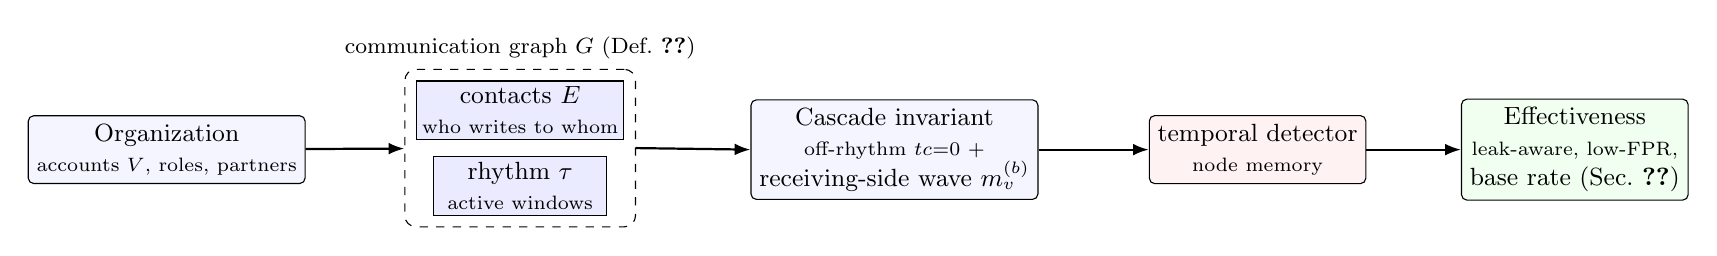
\begin{tikzpicture}[>=Latex, font=\small, node distance=6mm,
  box/.style={draw, rounded corners=2pt, align=center, minimum height=8mm, inner sep=3pt, fill=blue!4},
  lay/.style={draw, align=center, minimum width=22mm, minimum height=6mm, inner sep=2pt, fill=blue!8},
  det/.style={box, fill=red!5}, flow/.style={-{Latex[length=2mm]}, thick}]
  \node[box] (org) {Organization\\\scriptsize accounts $V$, roles, partners};
  \node[lay, right=14mm of org, yshift=5mm] (l1) {contacts $E$\\\scriptsize who writes to whom};
  \node[lay, below=2mm of l1] (l2) {rhythm $\tau$\\\scriptsize active windows};
  \node[box, right=16mm of l1, yshift=-5mm] (inv) {Cascade invariant\\\scriptsize off-rhythm $tc{=}0$ $+$\\receiving-side wave $m_v^{(b)}$};
  \node[det, right=14mm of inv] (d) {temporal detector\\\scriptsize node memory};
  \node[box, right=12mm of d, fill=green!6] (eff) {Effectiveness\\\scriptsize leak-aware, low-FPR,\\base rate (Sec.~\ref{sec:effectiveness})};
  \node[draw, dashed, rounded corners, fit=(l1)(l2), inner sep=4pt, label=above:{\footnotesize communication graph $G$ (Def.~\protect\ref{def:cg})}] (cg) {};
  \draw[flow] (org) -- (cg);
  \draw[flow] (cg.east) -- (inv.west);
  \draw[flow] (inv) -- (d);
  \draw[flow] (d) -- (eff);
\end{tikzpicture}}
\caption[General model]{The model, general to detailed (left to right). An organization induces the
communication graph $G$ with a rhythm per account; a compromised account violates it by writing off-rhythm
and by propagating, which leaves a receiving-side wave; a temporal detector with node memory reads that wave,
and is judged by one \emph{definition of effectiveness}.}
\label{fig:model}
\end{figure}

\begin{table}[pos=tbp]\centering\small
\caption{Notation used throughout the paper. Concrete instantiations of the free
parameters ($N$, $T$, $p_\mathrm{inf}$, $H$) are given in the Case Study (Sec.~\ref{sec:results}).}
\label{tab:notation}
\begin{tabular}{ll}
\toprule
\textbf{Symbol} & \textbf{Meaning} \\
\midrule
$G=(V,E,\tau)$ & organizational communication graph with rhythm \\
$V$ & set of accounts (people/roles), $|V|=N$ \\
$E$ & contacts: $(s,v)\in E$ iff $s$ corresponds with $v$ \\
$\tau(s)$ & temporal rhythm (active windows) of sender $s$ \\
$T$ & number of time buckets partitioning the period \\
$b$ & a single time bucket, $b\in\{1,\dots,T\}$ \\
$tc(s,v,t)$ & temporal consistency of $(s,v)$ at time $t$ \\
$s,v$ & sender, victim (recipient); $s_0$ the compromised account \\
$p_\mathrm{inf}$ & per-contact infection probability of a cascade \\
$H$ & maximum cascade depth (hops) \\
$K$ & number of carriers of a stealthy attacker (one send per bucket) \\
$Z$ & static-GNN node embedding matrix, Eq.~\eqref{eq:static} \\
$d_v^{(b)}$ & in-degree of node $v$ within bucket $b$, Eq.~\eqref{eq:temp-mem} \\
$m_v^{(b)}$ & temporal-GNN memory of node $v$ after bucket $b$ \\
\bottomrule
\end{tabular}
\end{table}

\subsection{The organizational communication graph}
\label{sec:cg}
An organization's communication is relational and rhythmic: who corresponds with whom follows the
organizational chart (supervisors, coworkers, business partners), and each account is active in
characteristic windows of the week. Both facts are observable from mail headers alone, without content.

\begin{definition}[Organizational communication graph]
\label{def:cg}
A communication graph is $G=(V,E,\tau)$, where $V$ is the set of accounts (people/roles), $E\subseteq V\times V$
is the set of contacts ($(s,v)\in E$ iff $s$ corresponds with $v$; induced by the organization's hierarchy,
coworker, and partner relations), and $\tau:V\to\mathcal{T}$ assigns to every sender a \emph{temporal
rhythm}, the set of its active time windows. The temporal consistency of a message from $s$ to $v$ at time
$t$ is $tc(s,v,t)=\mathbf{1}[t\in\tau(s)]$.
\end{definition}

\noindent A message from a known contact in its rhythm, $(s,v)\in E$ and $tc=1$, is the normal case. A known
contact writing \emph{off-rhythm}, $tc=0$, is the canonical signature of a compromise: the relation is
genuine, the timing is not. This single bit is weak on its own (legitimate mail also arrives off-hours, and an
attacker with mailbox access can mimic the rhythm), which is why the invariant below reads the dynamics of the
whole neighborhood rather than one message.

\subsection{Threat model: the compromised account}
\label{sec:threat}
The attacker has gained mailbox access to an internal account $s_0$ (the \emph{patient zero}) and wants to
deliver to victims messages classified as legitimate. From $s_0$ the attacker mails the account's own
contacts; each recipient becomes a carrier with probability $p_\mathrm{inf}$ and propagates to its own
contacts, up to depth $H$. The attack is therefore a \emph{cascade} on $G$ (Fig.~\ref{fig:cascade} in
Sec.~\ref{sec:method}). The term follows \citet{ho2019detecting}, who coined \emph{lateral phishing} for
phishing sent from compromised enterprise accounts and characterized it at scale; the multi-hop cascade with
a per-contact infection probability is our formalization of the compounding they observed, in which newly
compromised recipients become the next senders. Every single message in it is locally plausible: the sender is a genuine contact,
the address is real, and the content can be clean.

On capabilities: having mailbox access, the attacker knows the victim's rhythm and can mimic it; the attacker
can also \emph{pace} the sends---$K$ carriers, one send per time bucket---so that no sending burst ever appears
(the \emph{stealthy} attacker, who defeats volumetric detection by construction); and the attacker can restrict
the attack to a single recipient with no propagation at all (the \emph{surgical} attack). Out of scope is an
adaptive adversary with full knowledge of the graph and training poisoning, and external impersonation from
outside the graph, which requires knowledge beyond $G$ and is treated in a separate study. We treat the signal
as a cost increase for the attacker; no detection is final.

\subsection{The cascade invariant}
\label{sec:invariant}
Lateral phishing is a propagation process, and propagation has two sides. On the \emph{sending} side a
compromise shows up as a surge in one account's volume, or as an unusual path to a rare target; this is what
practical defenses read, and it is what a patient attacker controls. On the \emph{receiving} side the cascade
leaves a signature that no single message reveals and that the attacker cannot pace away: within the wave's
window many of $v$'s neighbors receive mail, and the sender $u$ of the message to $v$ was itself hit just
before. This receiving-side wave is the invariant. A learned temporal model with node memory registers it by
scoring an event using the state from \emph{before} its bucket, so that it can only use the past (made precise
in Sec.~\ref{sec:method}); a static model of the same topology, which sees who is connected to whom but not
in what order, cannot. The invariant is testable by ablation: shuffling the time order of events destroys
the order it relies on (together with within-bucket co-occurrence, Sec.~\ref{sec:m-detectors}), so the drop in
performance under a time shuffle bounds how much of the signal is dynamics rather than topology.

\subsection{Definition of detection effectiveness}
\label{sec:effectiveness}
Every result in the Case Study follows a standard that is detector-independent and operational; the
Methodology (Sec.~\ref{sec:method}) is the protocol that operationalizes it.

A high benchmark accuracy alone does not attest to detecting lateral phishing. A method works operationally
for the targeted tail only when its advantage is temporal, vanishing under a control that destroys the
temporal order, and transferable, so that the qualitative hierarchy of methods---which class wins, and where it
breaks down---carries over to other topologies. Effectiveness is judged by sensitivity at a low
false-positive rate with explicit base-rate accounting, rather than by headline AUC. The leak-aware protocol of
Sec.~\ref{sec:method} implements this standard.

% ============================================================
% Methodology — Paper A (JNCA): verification procedure for the cascade invariant.
% Procedure, variables, metrics, controls. NO concrete instantiation
% values (those live in the Case Study, Sec.~\ref{sec:results}).
% ============================================================
\section{Methodology}
\label{sec:method}

The procedure turns the cascade invariant into detectors, guards against inflated results, and checks the
metrics against the definition of effectiveness (Sec.~\ref{sec:effectiveness}). Concrete values---population,
time buckets, cascade parameters, hyperparameters---are stated once, in the Case Study (Sec.~\ref{sec:results}).

\subsection{Overview of the verification procedure}
\label{sec:m-overview}
The procedure has four steps that mirror the model. First, instantiate the communication graph $G$
(Def.~\ref{def:cg}) on a population, deriving the contacts $E$ and the temporal rhythm $\tau$. Then build
detectors of increasing temporal awareness, as standard learning instruments over graph-position features, and
two strong practical baselines that read the sending side. Evaluation follows under the leak-aware protocol
below, so that any advantage due to leakage or capacity is destroyed by a control; the last step checks
transfer to real topologies.

\subsection{Leak-aware evaluation protocol}
\label{sec:eval}
Graph detectors are easy to inflate, and the protocol below uses four safeguards against that.

A matched design makes legitimate traffic and attack edges share the same
distribution of endpoints and degrees, meaning they differ only by the temporal pattern and the
degree/identity confounder is removed \citep{arp2022dos}. A time-shuffle control permutes the temporal order of
events, which removes the advantage if it comes from dynamics and leaves it intact if it is an artifact of
topology or identity \citep{pendlebury2019tesseract}; an inductive split by organization checks that nothing is memorized about
the accounts seen in training, and an audit of noisy training labels checks that the learned detector does not
depend on clean labels. Operational metrics report sensitivity at a low FPR, with explicit base-rate
arithmetic, rather than relying on headline AUC alone. A \emph{predictivity probe} then asks whether what was established on one
topology carries over to another (real Enron, SNAP graphs). The probe checks two properties: that the
\emph{qualitative hierarchy} of detectors---which class wins, and in which attack regime it breaks down---is
reproduced on each real graph, and that the headline contrast (receiving-side signal vs.\ volume) keeps its
direction there; with the few seeds available per real graph this is a directional check, not a
significance test. We deliberately do not reduce the probe to a single rank-correlation
coefficient: over a handful of detectors such a coefficient is underpowered, and the transferable claim is the
regime-level contrast, not a full ranking. Together these give the working definition of effectiveness of
Sec.~\ref{sec:effectiveness}: a method works when its advantage meets the standard defined there.

\subsection{Detectors and causal controls}
\label{sec:m-detectors}
The design principle is uniform: features encode graph position and timing, never identity. This makes every detector
inductive and applicable to accounts unseen in training.

\smallskip The invariant operates on the contacts graph
$G=(V,E)$ with time divided into $T$ buckets. An attack is a cascade where a patient-zero $s_0$ sends malicious mail
to contacts; each recipient becomes a carrier with probability $p_\mathrm{inf}$ and propagates to depth $H$
(Fig.~\ref{fig:cascade}). A single event $u\!\to\!v$ is locally indistinguishable from legitimate mail; the
signal is the cascade context, since within the wave's window many of $v$'s neighbors receive mail and $u$ was
hit just before. Four detectors of increasing temporal awareness are compared: a 1-hop tabular model (a lower
bound), a hand-crafted cascade context (1-hop plus burst, freshness, and wave density), a static GNN (topology,
no time), and a temporal GNN with node memory.
% ZMIANA: dodano opis treningu w eksperymencie stealth: kazdy poziom K to osobne zadanie,
% detektor uczy sie i jest sprawdzany w jednym reżimie. Powod: bez tej informacji czytelnik
% mogl podejrzewac, ze zly wynik detektora wolumetrycznego bierze sie z rozjazdu miedzy
% daniem treningowym a testowym.
In the stealth experiment each regime is a self-contained
training task: for every stealth level $K$ the scenario (attack plus matched benign) is generated, the split is
victim-disjoint, and every detector is trained and tested \emph{within that regime only}---no detector ever
sees a mixture of regimes, so its collapse or survival is a property of the regime, not of a train--test
regime shift.

\smallskip The two equations below differ in one respect: whether the model may
look forward in time. The static score summarizes a node by its neighbors in the whole aggregated graph, seeing
who is connected to whom but not in what order. The temporal score keeps a running memory updated
in event order and read from the state before the event it scores, so its memory can only use the past.
% ZMIANA (A1, recenzja wewnetrzna r2): zasada przeczynowosci przepisana z kubełkowej
% (<= b-1) na ZDARZENIOWA — wszystkie detektory widza wylacznie zdarzenia o scisle
% wczesniejszym t(e) = (kubelek, pozycja na liscie). Powod: podzial kubełkowy ukrywal
% fale budujaca sie w biezacym kubełku (asymetria faworyzujaca volume pod blastem);
% regula remisow: porzadek tasowanej listy zdarzen, ustalony per przebieg. TGN czyta
% pamiec per mini-batch (<=64 zdarzen w kubełku) — batch jest wspolczesny. Test
% anty-wyciek: tests/test_causality.py (cechy/logity niezmienne po usunieciu zdarzen
% o czasie >= t(e)).
This rule is enforced uniformly across the whole detector panel (A1): every stream-derived
feature---the volumetric counters, the burst/freshness/propagation windows of the hand-crafted context,
and the precursor/momentum/rare-target components of the path-based baseline---is computed from events
with a strictly smaller total timestamp $t(e)=(b,\text{position})$ only, where the position is the fixed
(shuffled) stream order used as the tie rule within a bucket; the temporal GNN's memory is likewise
updated per mini-batch of at most $64$ simultaneous events in that order, each scored from the state
before it, and the GNNs' static node features (in-/out-degree) are computed from the
\emph{training} split only. Earlier drafts of the package computed some of these features on the full
event stream, and a later draft split causality at bucket boundaries; both hid parts of the signal and
the latter made the baselines asymmetric, so all experiments were
re-run under the uniform event-causal rule and the numbers in this manuscript come from the fixed package.
That past-only
reading is what lets the receiving-side wave become a signal, and it is what a time-shuffle destroys.

\smallskip The static GNN builds embeddings from the aggregated graph with a normalized
adjacency $\hat{A}$ and features $X$,
\begin{equation}
Z = \hat{A}\,\sigma\!\big(\hat{A}\,X\,W_1\big)\,W_2,
\qquad
\mathrm{score}_{\mathrm{stat}}(s,v) = g\!\big([\,Z_s,\,Z_v,\,Z_s\!\odot\!Z_v,\,x_{sv}\,]\big),
\label{eq:static}
\end{equation}
whereas the temporal GNN maintains a memory $m_v$ and scores an event from the memory state
immediately before it in event order, which preserves causality and avoids leakage,
\begin{align}
\mathrm{score}_{\mathrm{temp}}(s,v,e) &= g\!\big([\,m_s^{(<t(e))},\,m_v^{(<t(e))},\,m_s^{(<t(e))}\!\odot\!m_v^{(<t(e))},\,x_{sv}\,]\big),
\label{eq:temp-score}\\
m_v^{(k)} &= \mathrm{GRU}\!\Big(\tfrac{1}{d_v^{(k)}}\!\!\sum_{u:\,(u\to v)\in B_k}\!\!\sigma\!\big(W_m\,m_u\big),\; m_v^{(k-1)}\Big),
\label{eq:temp-mem}
\end{align}
where $B_k$ is the $k$-th mini-batch of events in total time order and $d_v^{(k)}$ the number of its
messages received by $v$ (a normalizer for the mean-pooled message).

The shuffle control is a temporal ablation. Since $\mathrm{score}_{\mathrm{stat}}$ is permutation-invariant in
time while $\mathrm{score}_{\mathrm{temp}}$ is not, the drop in $\mathrm{AUC}_{\mathrm{temp}}$ after time
shuffling indicates how much the model relies on temporal order. The ablation is not perfectly selective:
shuffling also breaks the co-occurrence of events within a bucket, so the drop is an upper bound on the
contribution of order alone (consistent with the shuffled temporal model falling slightly below the static
GNN, Tab.~\ref{tab:detectors}). We use ``causal'' in this ablation sense throughout, not in the sense of
causal identification.

\smallskip Beyond the GNN we implement two strong practical methods, both of which read the sending side.
\begin{itemize}[noitemsep,topsep=2pt]
  \item A volumetric baseline inspired by COMPA \citep{egele2013compa,stringhini2015thataint} scores an event
  by the sender's deviation from its own volume profile---how unusual the recipient, the time bucket, and the
  sender's overall activity are (three per-event features, Supplementary Sec.~S6)---with the same
  gradient-boosting learner as the other tabular detectors,
  \item and a path-based baseline that transfers the causal-path idea of Hopper \citep{ho2021hopper}, a
  detector of lateral movement in login graphs, to the email graph: it looks for a causal precursor,
  momentum, and a rare target.
\end{itemize}
We implement their structural-temporal core rather than the full systems, which is why we label them ``volumetric'' and
``path-based''; the exact feature set of every detector is listed in Supplementary Sec.~S6, together with what
the full systems add on top. Hyperparameters of all detectors are fixed uniformly, without intensive tuning,
so that no detector enjoys a tuning advantage; the concrete settings are given in Supplementary Tab.~S1.

\begin{figure}[pos=tbp]\centering
\resizebox{0.92\textwidth}{!}{%
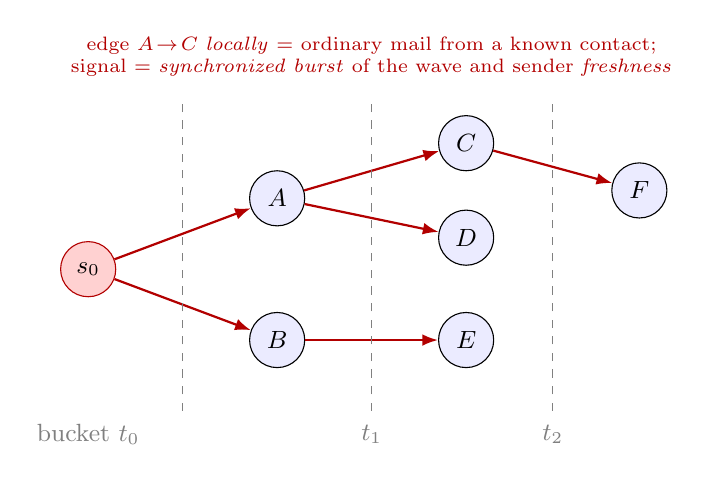
\begin{tikzpicture}[>=Latex, every node/.style={font=\small},
  acc/.style={circle, draw, minimum size=7mm, inner sep=1pt},
  inf/.style={acc, fill=red!18, draw=red!70!black},
  ben/.style={acc, fill=blue!8},
  mal/.style={-{Latex[length=2mm]}, red!70!black, thick}]
  \node[inf] (p) at (0,0) {$s_0$};
  \node[ben] (a) at (2.4,0.9) {$A$};
  \node[ben] (b) at (2.4,-0.9) {$B$};
  \draw[mal] (p)--(a); \draw[mal] (p)--(b);
  \node[ben] (c) at (4.8,1.6) {$C$};
  \node[ben] (d) at (4.8,0.4) {$D$};
  \node[ben] (e) at (4.8,-0.9) {$E$};
  \draw[mal] (a)--(c); \draw[mal] (a)--(d); \draw[mal] (b)--(e);
  \node[ben] (f) at (7.0,1.0) {$F$};
  \draw[mal] (c)--(f);
  \node[gray] at (0,-2.1) {bucket $t_0$};
  \node[gray] at (3.6,-2.1) {$t_1$};
  \node[gray] at (5.9,-2.1) {$t_2$};
  \draw[gray, dashed] (1.2,-1.8) -- (1.2,2.1);
  \draw[gray, dashed] (3.6,-1.8) -- (3.6,2.1);
  \draw[gray, dashed] (5.9,-1.8) -- (5.9,2.1);
  \node[red!70!black, align=center, font=\scriptsize] at (3.6,2.7)
    {edge $A\!\to\!C$ \emph{locally} = ordinary mail from a known contact;\\
     signal = \emph{synchronized burst} of the wave and sender \emph{freshness}};
\end{tikzpicture}}
\caption[Lateral phishing as a temporal cascade]{Lateral phishing as a temporal cascade: a carrier ($s_0$)
infects contacts, and those in turn infect their own, so the wave propagates across the graph. Detection requires \emph{multi-hop,
temporal} propagation context.}
\label{fig:cascade}
\end{figure}

\subsection{Event model and data split}
\label{sec:m-events}
An event is a pair (sender $s$, victim $v$) with a bucket $b$, labeled legitimate or attack, with two-sided noise so
that the classes are not perfectly separable. Legitimate events are messages between known contacts in rhythm,
with a fraction arriving off-rhythm (an irreducible source of false positives). Attacks are the events of a
cascade seeded at a compromised account, a fraction of which mimic the sender's rhythm. We use two split
regimes, victim-wise (disjoint victim sets) and organization-wise (test organizations disjoint from training
ones, an inductive validation). Headline claims are hardened over many seeds; validations on real graphs use
fewer seeds, since variance is lower on a fixed structure, with a Wilcoxon test where significance matters.
Seed counts for each experiment are given in the respective table or figure caption.

\subsection{Metrics, base rate, and threats to validity}
\label{sec:m-metrics}
The headline metric is sensitivity at a fixed low FPR, the operational working point,
$\text{sensitivity}@\mathrm{FPR} = \max\{\mathrm{TPR}(\theta):\mathrm{FPR}(\theta)\le\alpha\}$ (where $\alpha=0.01$ for our primary analysis); AUC is reported
alongside it. Real systems operate at a far stricter FPR ($<\!4$~FP/million, \citep{ho2019detecting}), so the FPR
reported here (an FPR of $10^{-2}$ against $4\cdot10^{-6}$) is a liberal operating point rather than a
deployment threshold; at a realistic prevalence, precision
follows from Bayes' theorem, which we make explicit in the Case Study (Sec.~\ref{sec:res-rigor}). To isolate the
signal we use the temporal-order shuffle as the causal control: if the signal is truly dynamic, the control
must destroy the advantage.

\smallskip\noindent\textbf{Threats to validity.} The internal threats are label leakage, which we counter by
separating features from the hidden infection state and letting the shuffle control isolate the mechanism, and
dependence on the cascade parameters, which we counter by sweeping the infection probability and depth
(Supplementary Tab.~S2). The external threat is that the maliciousness is synthetic, so we validate the mechanism on
real Enron and two SNAP graphs under controlled injections; the synthetic data lets us control the cascade at
the cost of absolute effects. The construct threat is addressed by preferring sensitivity at low FPR to
headline AUC, in line with \citep{arp2022dos,pendlebury2019tesseract}.

% ============================================================
% Case Study and Results — Paper A (JNCA): the organizational case study,
% the cascade invariant, real-graph replication, rigor.
% All numbers are copied verbatim from the reproducibility package.
% ============================================================
\section{Case Study and Results}
\label{sec:results}

The \emph{case study} defines the organizational population, the communication graph with its rhythm, and the
cascade parameters that instantiate $G$, providing the concrete values for the symbols in
Sec.~\ref{sec:model}.

% ============================================================
\subsection{Case study: the organization and what is tested on it}
\label{sec:cs-setup}
The case study is a fully specified organizational ecosystem (Fig.~\ref{fig:casestudy}): $19$~firms from
distinct sectors (a bank, a hospital group, a software house, a law firm, a logistics company, an insurer,
a public office, \dots), each a small office of $\sim\!8$~accounts with one managing director, one senior
manager, and five to six specialists and analysts ($19$/$19$/$57$/$55$ accounts in the four seniority
levels). Everyone in a firm corresponds with everyone else in it, and the firms are tied into a ring of
business partnerships (director to director, plus one specialist counterpart per partnership), which gives
$N{=}150$ accounts and $556$ contact edges ($518$ inside firms, $38$ between partner firms). The population is
synthetic, but it is generated \emph{graph-first}: the organization graph is designed deterministically and
each persona is then generated \emph{in its node}, so that a persona's supervisor, coworkers, and external
contacts are \emph{real other personas} with real corporate addresses, and the graph closes internally. The
% ZMIANA: dodano opis budowy grafu Enron: bierzemy nagłówki Od/Do/Kopia i 2000
% najaktywniejszych kont (zostaje 1990). Wyjasniono tez roznice z artykulem B (818 nadawcow):
% tam potrzebny jest rytm kazdego nadawcy, wiec odrzucani sa nadawcy z mniej niz 25 mailami.
% Powod: bez tego 818 vs 1990 z tego samego korpusu wyglada na blad.
size $N{=}150$ is of the order of the core user set of the Enron corpus \citep{klimt2004enron}; the Enron
contacts graph used for validation (Sec.~\ref{sec:res-realgraphs}) is larger (${\approx}1970$~accounts), so the
real-graph replication also tests the mechanism at a larger scale; anomaly analysis of this corpus as a
communication graph has a long precedent, from scan statistics over Enron graphs \citep{priebe2005scan} onward. That graph is built from the
\texttt{From}/\texttt{To}/\texttt{Cc} headers of the maildir corpus as an undirected sender--recipient graph;
we keep the $2000$ highest-degree accounts and remove nodes left isolated by this filter, which leaves
${\approx}1970$~accounts. A companion study of the external-impersonation mode uses $818$~senders from the same corpus: its
multiplex requires a per-sender rhythm, so it keeps only senders with at least $25$~messages and a
non-empty active-bucket set; the difference is therefore a filter serving a different construction
(topology breadth here, per-sender temporal profiles there), not an inconsistency.

We divide the week into $T{=}28$ buckets (7~days $\times$ 4~six-hour blocks); an account's rhythm $\tau$ is the
set of its active buckets ($6$ per persona synthetically; on Enron derived from the \texttt{Date} headers).
Realistic noise: $15\%$ of legitimate mail arrives off-rhythm and $25\%$ of attacks mimic the rhythm. For the
cascade (Sec.~\ref{sec:m-detectors}) the per-contact infection probability is $p_\mathrm{inf}{=}0.6$ and the
maximum depth is $H{=}4$. Detector hyperparameters are fixed uniformly (Supplementary Tab.~S1).

\paragraph{What the case study tests} One kind of attack is injected into this graph, in three regimes
(Fig.~\ref{fig:casestudy}). A \emph{compromised internal account} $s_0$ mails its own contacts off-rhythm;
each recipient becomes a carrier with probability $p_\mathrm{inf}$, so the attack spreads as a cascade that
crosses into the partner firm through the business-partnership edge. The sender is a genuine contact
consistent with every static relation, so only the timing and the receiving-side wave give it away, and this
is what T1 must catch. Beyond the default cascade we probe three \emph{extreme} regimes, each chosen to stress
% przyczynowosc zdarzeniowa (liczniki widza wczesniejsze zdarzenia TEGO kubełka) blast
% jest znowu wygrana detektora wolumetrycznego (0.83 na SNAP, 0.63 na grafie case
% study) — i wlasnie dlatego reżim skryty jest tym, ktory go lamie: te same liczniki
% nie maja czego liczyc, gdy nosiciel wysyla raz na kubełek.
a specific claim rather than to represent typical traffic. \emph{(i)~Naive blast}: one carrier infects all
contacts at once, the maximally bursty case and the easy end of the scale---with event-causal counters the
volumetric detector \emph{does} catch it (AUC $0.83$ on the SNAP blast regimes, Tab.~\ref{tab:realgraphs}),
which is exactly what makes the stealthy regime the informative one.
\emph{(ii)~Stealthy spread} ($K$~carriers, one send per interval, down to $K{=}1$): the burst is smeared out,
so this is the case that \emph{breaks} volume detection and isolates the receiving-side signal.
\emph{(iii)~Single-recipient surgical attack} ($p_\mathrm{inf}{=}0$, fan-out~$1$): no propagation at all,
the \emph{blind spot} that no cascade detector can see, included to mark the lower boundary of the threat
model (T2). The stealthy-attacker and baseline contrasts are averaged over $20$ random seeds on synthetic
data and the detector hierarchy over $5$; real-graph validations use $8$ (Enron) and $3$ (SNAP) seeds.
Seed counts are stated in every caption.

\begin{figure}[pos=tbp]\centering
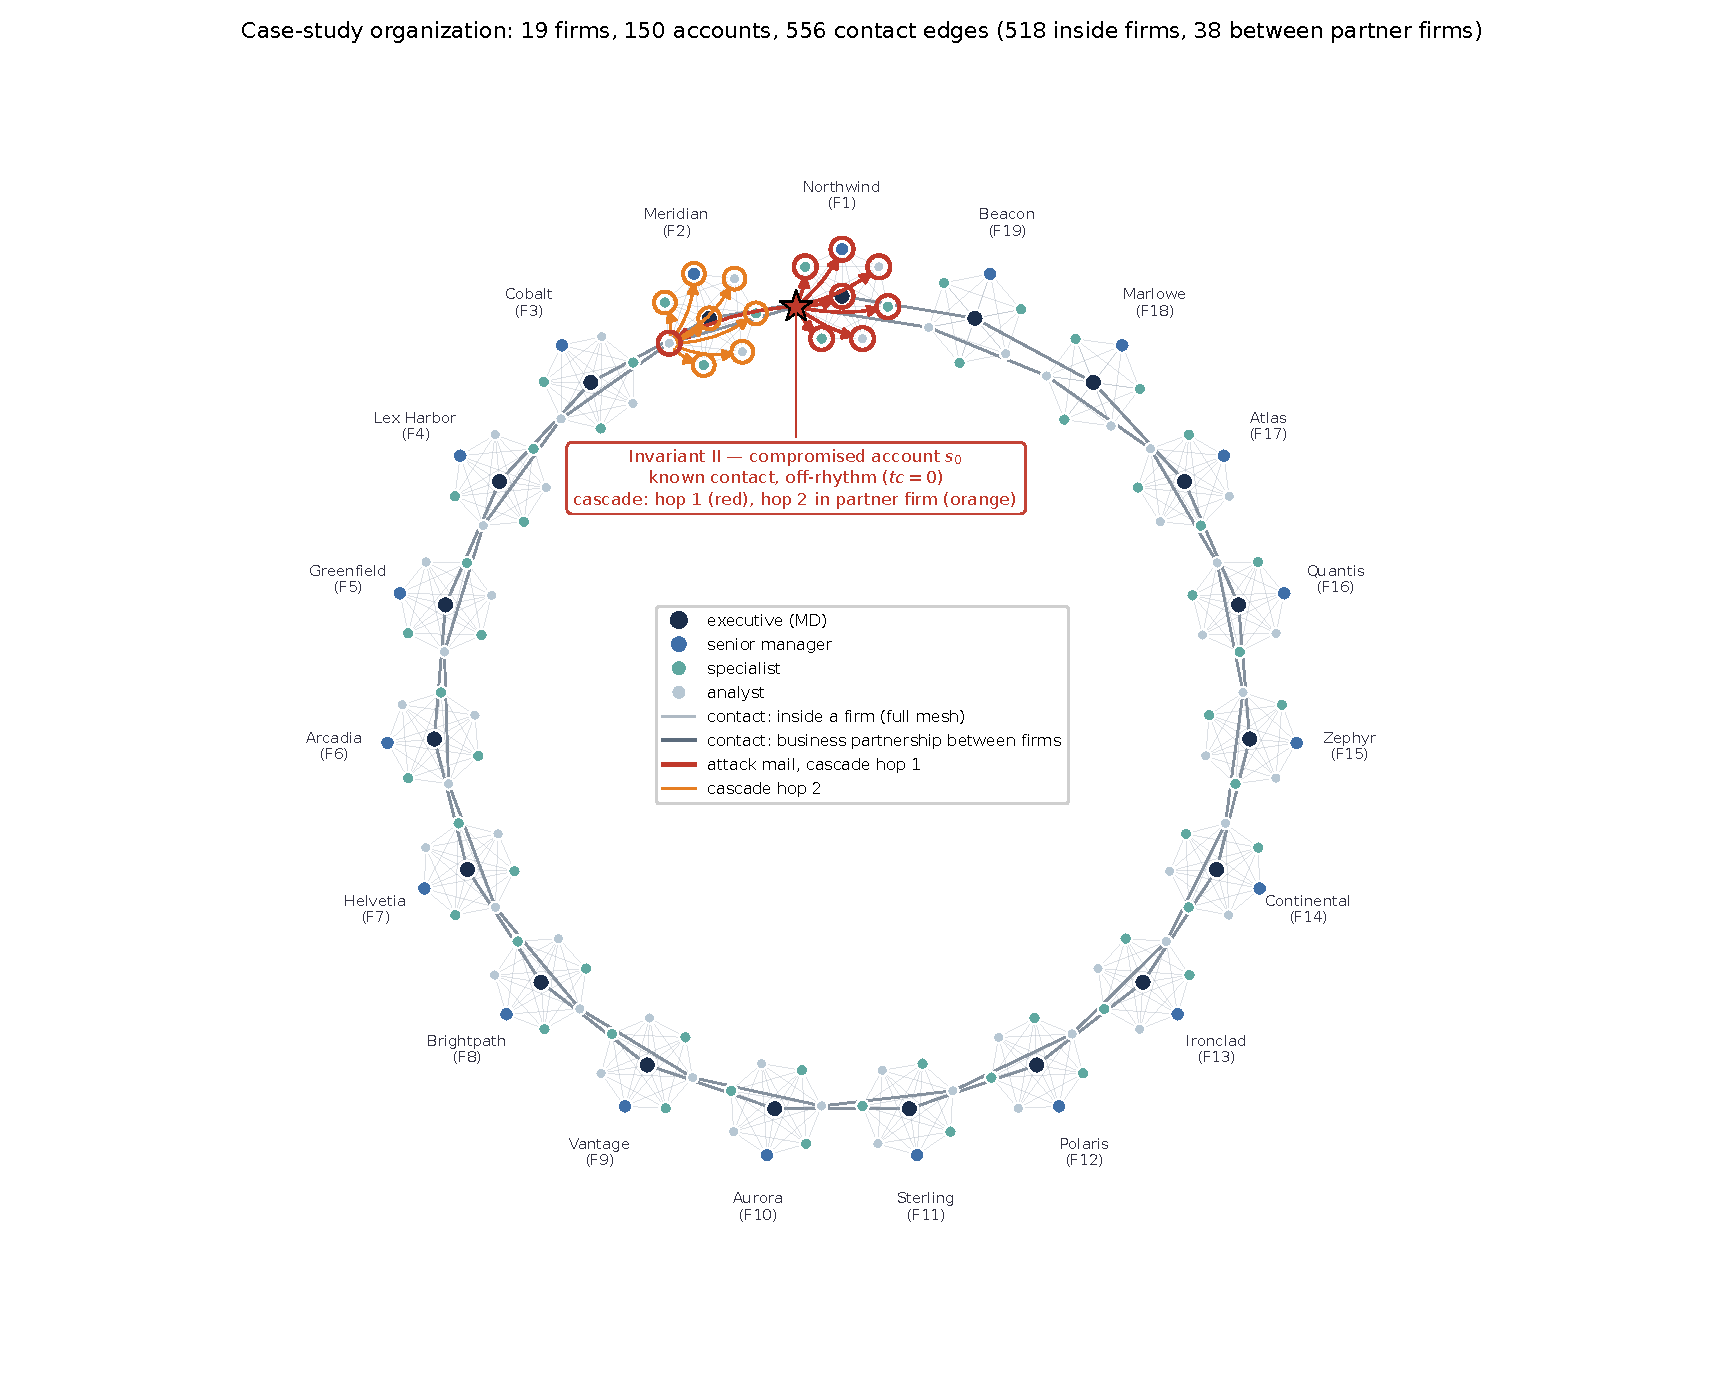
\includegraphics[width=\linewidth]{fig_org_case_study_cascade.pdf}
\caption[Case-study organization]{The case-study organization, drawn from the population data of the
reproducibility package: $19$~firms on a ring of business partnerships, $150$~accounts colored by seniority,
and the real contacts layer ($556$~edges). Overlaid is the attack the detectors must catch: a compromised
account $s_0$ (star) whose off-rhythm mail cascades through its own firm (hop~1, red) and into the partner
firm through the business-partnership edge (hop~2, orange). Every message in the cascade comes from a genuine
contact; only the timing and the receiving-side wave reveal it.}
\label{fig:casestudy}
\end{figure}

% ============================================================
\subsection{Results overview}
\label{sec:res-overview}
Table~\ref{tab:roadmap} maps the two research questions of Sec.~\ref{sec:intro} to the evidence; the
subsections follow that order. Results are reported on a victim or organization split, as AUC and, where
the operating point matters, sensitivity@FPR$1\%$; the time-shuffle control is applied to the detector
hierarchy on the case-study graph and on Enron. Seed counts are stated in each table or figure caption.

\begin{table}[pos=htbp]\centering\small
\begin{tabular}{@{}l p{0.29\linewidth} p{0.36\linewidth} p{0.22\linewidth}@{}}
\toprule
& \textbf{Sub-thesis} & \textbf{Main evidence} & \textbf{Verdict} \\
\midrule
RQ1 & the receiving-side cascade signal detects a compromise and stays above volume under a stealthy attacker (T1) &
Tabs.~\ref{tab:detectors}--\ref{tab:baselines}(a); real graphs: Tab.~\ref{tab:realgraphs};
Secs.~\ref{sec:res-detectors}--\ref{sec:res-baselines}, \ref{sec:res-realgraphs} &
stays above volume at every stealth level; vanishes under time shuffle; replicates in direction on three real graphs \\
\addlinespace
RQ2 & the signal needs fan-out~$\ge2$, degrades gracefully, and is a triage instrument at a real base rate (T2) &
Tab.~\ref{tab:baselines}(b); Supplementary Tabs.~S3--S4; Tab.~\ref{tab:baserate};
Secs.~\ref{sec:res-baselines}, \ref{sec:res-stability}, \ref{sec:res-rigor} &
fan-out~$\ge2$ needed; graceful under noise and scale; triage, not autonomous defense \\
\bottomrule
\end{tabular}
\caption{Map from research questions to evidence. Each verdict is established in the section listed.}
\label{tab:roadmap}
\end{table}

% ============================================================
\subsection{The cascade detectors}
\label{sec:res-detectors}
% ZMIANA: wszystkie liczby policzono od nowa po naprawie kodu. Dodano wiersz 'Library TGN'
% z brakujacymi liczbami (oficjalna implementacja z biblioteki PyG). Usunieto zdanie o
% 'AUC 0.49 detektora statycznego' — 0.49 to wynik innego eksperymentu (pelna slepota
% cech statycznych pod przejeciami kont), nie tej tabeli. Dodano zdanie, ze przewaga GNN
% nad kontekstem recznym dotyczy tylko zwyklej kaskady — w reżimie skrytym oba sa rowne.
A compromised account passes every static relation, so static graph position alone carries little
operational signal (the static GNN reaches AUC $0.76$ but only $0.039$ sensitivity at FPR~$1\%$). The
signal must therefore lie in the dynamics. Table~\ref{tab:detectors} tests T1 on the default cascade of
Fig.~\ref{fig:casestudy} and shows a clear hierarchy among detectors (bar chart in Supplementary Fig.~S1):
local 1-hop features are essentially useless (AUC $0.70$, sensitivity@FPR$1\%\!\approx\!0$), while a
hand-crafted multi-hop context reaches $0.81$. A static GNN captures the topology but misses the timing
($0.76$), and the volumetric baseline---evaluated in the same pass---ranks the naive cascade at $0.83$
but converts it into a worse operating point than the temporal model ($0.23$ vs $0.10$ sensitivity at
FPR~$1\%$), leaving the temporal GNN in the lead (AUC $0.87$, sensitivity@FPR$1\%$ $0.099$). This lead is
specific to the default cascade: under the stealthy regime of the second harness the temporal GNN and the
hand-crafted context are statistically indistinguishable (Sec.~\ref{sec:res-rigor}). This advantage is
temporal in the ablation sense. A simple time permutation drops the temporal GNN back to the static level
($0.87\!\to\!0.73$, sensitivity $0.099\!\to\!0.022$). Architecture choice matters less than the paradigm;
TGN-lite and TGAT-lite outperform the hand-crafted context ($0.87$ and $0.88$ vs $0.81$ AUC;
Supplementary Sec.~S1), and the library TGN
\citep{rossi2020temporal} reaches $0.79$ AUC with $0.112$ sensitivity@FPR$1\%$---below our TGN-lite on
AUC but close to it on the operational metric (the library-TGN row of Tab.~\ref{tab:detectors}, $3$~seeds).

\begin{table}[pos=tbp]\centering
\begin{tabular}{lcc}
\toprule
Detector & AUC & sensitivity@FPR$1\%$ \\
\midrule
\csname @@input\endcsname tables/tab_detectors 
\bottomrule
\end{tabular}
% ZMIANA: tabele generowane teraz bezposrednio z CSV (analysis/gen_tables.py) — nikt
% nie przepisuje liczb recznie. Dodano wiersz volumetric (COMPA) w tym samym przebiegu
% (A3) i wszystkie detektory dostaly jedna regule przyczynowosci zdarzeniowej (A1).
\caption{Cascade detectors on the case-study graph (victim split, $5$~seeds; library TGN row: $3$~seeds):
only the temporal models with node memory reach operational sensitivity ($0.099$ and $0.112$ at FPR~$1\%$),
the volumetric baseline ranks the naive cascade well ($0.83$) but converts it to a worse operating point
than the temporal GNN ($0.23$ vs $0.10$ at a much noisier threshold), and
shuffling the time order removes the temporal advantage ($\to\!0.73$), so the signal depends on temporal order.}
\label{tab:detectors}
\end{table}

% ============================================================
\subsection{The stealthy attacker}
\label{sec:res-stealth}
% ZMIANA: liczniki wolumetryczne przepisano na przyczynowosc na poziomie ZDARZENIA
% (patrza na wczesniejsze zdarzenia TEGO samego kubełka, nie tylko na wczesniejsze
% kubełki). Powod: recenzent zauwazyl, ze przy podziale na poziomie kubełka detektor
% wolumetryczny w ogole nie widzi rozwijajacego sie burstu — to czynilo go slomiana
% kuka, a to byloby zbyt latwe twierdzenie. Po naprawie volume widzi burst (w blast
% AUC 0.63; w harnessu SNAP nawet 0.83), ale w reżimie skrytym nadal nie ma z czego
% liczyc sygnalu: jedno wyslanie na kubełek zostawia puste KAZDE okno przyczynowe.
% Dodano wiersz 'rhythm-only' i udzialy poczty poza rytmem: ataki 75-79%,
% legalna 78-79% — sam bit rytmu nie odróżnia tu niczego. Liczby 15%/25% naleza do
% generatora artykulu B, nie tu.
Table~\ref{tab:stealth} is the headline test of T1: the stealthy attacker breaks volume, but not dynamics.
Against an attacker who evades detection by spreading its sends over time ($K$~carriers, one per interval),
the volume detector never develops a usable signal (AUC $0.50$--$0.63$ across all levels---its event-causal
counters now see the burst that builds up within a bucket, but one send per bucket leaves every causal
window empty), while the temporal GNN stays above it
at every level (AUC $0.59$, sensitivity@FPR$1\%$ $0.026$ vs $0.000$ for volume at $K{=}1$) because it
picks up the receiving side of the cascade.
% ZMIANA jezykowa: 'the volume detector breaks down ... while the temporal GNN degrades less' przepisano —
% powod: w liczbach absolutnych temporal traca WIECEJ niz volume (0.86->0.59 vs 0.63->0.50 od blast
% do K=1); prawdziwe twierdzenie brzmi 'temporal jest powyzej volume na kazdym poziomie K'.
Each detector is trained and tested within a single $K$~regime on a victim-disjoint split (Sec.~\ref{sec:m-detectors}),
so the volumetric weakness is not a train--test regime shift. We also report a rhythm-only control: in this
harness the off-rhythm share is nearly identical for attacks ($75$--$79\%$) and for legitimate traffic
($78$--$79\%$), because the benign buckets are drawn uniformly and the attack buckets consecutively, so the
rhythm bit alone stays at chance ($0.50$--$0.54$) and none of the signal can be attributed to it; the
$15\%/25\%$ rhythm parameters quoted in Sec.~\ref{sec:cs-setup} belong to the companion study's persona
generator, not to this harness. At $K{=}1$ the temporal signal is weak in absolute terms, and the hand-crafted context is
the strongest single detector ($0.73$, sensitivity $0.11$); the claim is the relative one---the receiving-side signal does not
collapse---which Table~\ref{tab:baselines} then qualifies. The temporal sensitivity
column is not monotone in $K$ ($0.026 \to 0.051 \to 0.042 \to 0.044$ from $K{=}1$ to $K{=}5$) while the corresponding AUC rises monotonically from
$K{=}2$ on ($0.74 \to 0.74 \to 0.76$); we attribute the non-monotonicity to seed-level variability of the low-FPR operating point,
which depends on a tail quantile of the score distribution, rather than to a change in mechanism.

\begin{table}[pos=tbp]\centering
% ZMIANA: dodano kolumne kontekstu recznego — powod: przy K=1 to on jest najlepszym detektorem
% (0.72 AUC, czulosc 0.097) i ukrywanie go w tekscie czynilo teze o GNN silniejsza niz dane.
\begin{tabular}{lcccccc}
\toprule
& \multicolumn{3}{c}{AUC} & \multicolumn{3}{c}{sensitivity@FPR$1\%$} \\
\cmidrule(lr){2-4}\cmidrule(lr){5-7}
Level & vol. & manual & temp. & vol. & manual & temp. \\
\midrule
\csname @@input\endcsname tables/tab_stealth 
\midrule
rhythm-only bit (all levels) & \multicolumn{3}{c}{$0.50$--$0.54$} & \multicolumn{3}{c}{$0.000$} \\
\bottomrule
\end{tabular}
% ZMIANA: liczby po przepisaniu wszytkich detektorow na przyczynowosc zdarzeniowa (A1)
% — pod atakiem skrytym (jedno wyslanie na kubelek) okna zdarzeniowe sa i tak puste,
% wiec kierunek bez zmian; kontekst reczny umocnil sie przy K=1 (czulosc 0.11).
\caption{Stealthy attacker on the case-study graph ($K$~carriers spread over time; $20$~seeds): the
volumetric detector is near chance at every level ($0.48$--$0.63$), the temporal GNN stays above it at
every level, and the hand-crafted context is the strongest detector at $K{=}1$ ($0.73$, sensitivity
$0.11$)---the headline result behind T1 is the receiving-side signal, read equally well by the learned
model and by the hand-crafted features, not the superiority of either. The
rhythm-only control stays at chance at every level, so the signal is the receiving-side wave, not the
rhythm bit.}
\label{tab:stealth}
\end{table}

Figure~\ref{fig:stealth} plots the same breakdown across $K$: both detectors weaken as the attack gets
stealthier, and the receiving-side signal keeps its margin over the volumetric one at every level.

\begin{figure}[pos=tbp]\centering
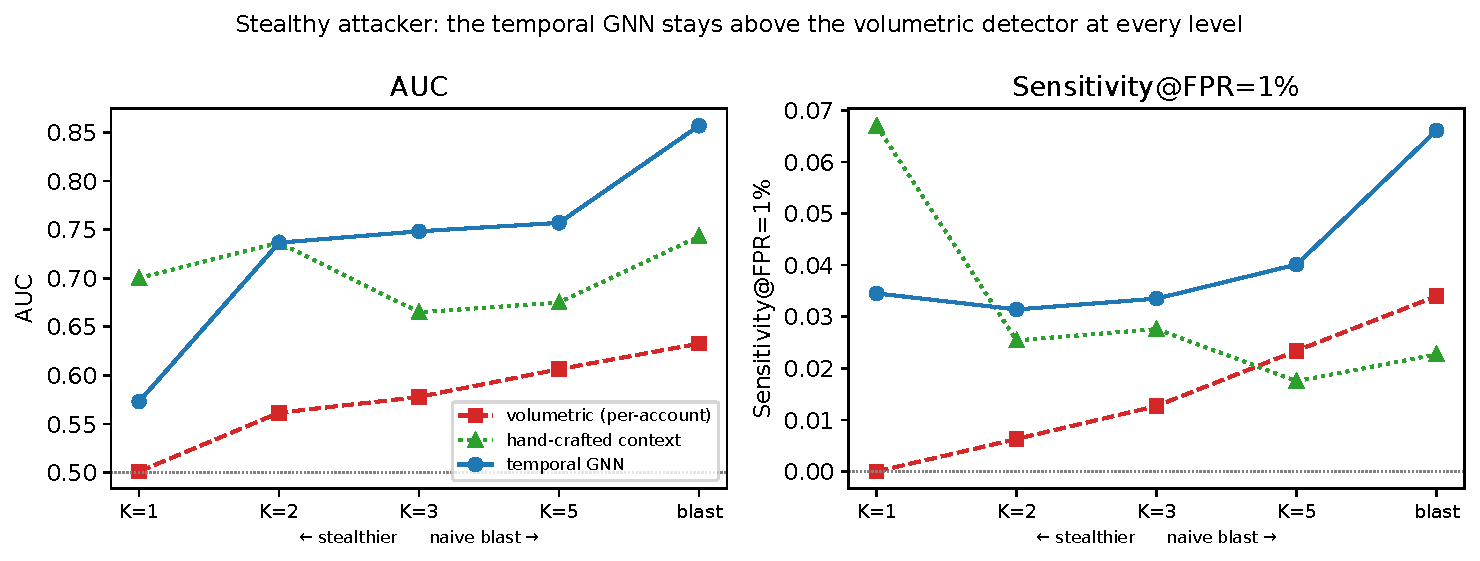
\includegraphics[width=\linewidth]{fig_cascade_stealth.pdf}
\caption[Stealth vs volume breakdown]{As the attack gets stealthier (smaller $K$) both detectors weaken,
but the temporal GNN keeps its margin over the volumetric one thanks to the cascade's receiving-side signal.}
\label{fig:stealth}
\end{figure}

% ============================================================
\subsection{Baselines and the boundary of the threat model}
\label{sec:res-baselines}
% ZMIANA: obie czesci tabeli wygenerowal na nowo odtworzony skrypt (oryginalnego
% brakowalo w paczce, wiec tabeli nie dalo sie odtworzyc; teraz 20 nasion losowosci).
% Dodano opis, czym roznia sie oba zestawy eksperymentow — bez tego to samo K dawalo
% rozne liczby i wygladalo to na blad. Wyjasniono tez wynik ~0.54 kontekstu recznego
% w ataku chirurgicznym: on liczy kontakte OFIARY trafione w przeszlych kubełkach,
% a atak jednokrotnie trafia wlasne kontakty nadawcy, wiec sasiedztwo ofiary
% nie jest odslane w oknie.
Table~\ref{tab:baselines} places this result against the two strong practical baselines and marks the boundary
of the threat model. This table comes from the second experiment harness (Supplementary Sec.~S6), so its
$K{=}1$ values differ slightly from Tab.~\ref{tab:stealth}. In the stealthy regime (block~a) the
path-based detector and the hand-crafted context lead under extreme stealth ($K{=}1$: $0.74$ and $0.77$,
ahead of the temporal GNN $0.63$) but degrade with reach (path $0.74\!\to\!0.65$), while the temporal GNN
has the largest end-to-end gain ($0.63\!\to\!0.85$) and leads from $K{=}3$ on. The two harnesses
differ in the generator and the population, not in the feature definitions: Tab.~\ref{tab:stealth} uses the
$150$-account case-study graph with consecutive-bucket stealth and uniform benign buckets, while
Tab.~\ref{tab:baselines} uses a $600$-account synthetic organization with an $8$-bucket send spacing,
$30\%$ rhythm mimicry, and $15\%$ off-rhythm benign traffic, plus a benign matched to the attack
(Sec.~\ref{sec:m-detectors}). Two remarks on reading this table. First, the path-based baseline keeps its
score although the look-ahead is removed: the corrected momentum counts \emph{past} targets---a different
signal, not a subset of the uncorrected one---and the harness uses its own generator, whose benign
protocol ($15\%$ off-rhythm, spread $8$, mimicry $0.3$) differs from the first harness, so part of the
difference against the stealth table is a harness difference, not only the causal fix. Second, the $K{=}1$ row has no
single winner among path-based and hand-crafted detectors ($0.74$ vs $0.77$); neither should be read as
the regime's best detector without per-seed intervals. The ablation column ``path (no precursor)''
answers the question of how much of the path baseline's stealth performance is carried by its precursor
feature, which largely coincides with the freshness bit of the hand-crafted context: zeroing it out
drops the path baseline by $0.06$--$0.12$ AUC at every stealth level ($0.74\!\to\!0.62$ at $K{=}1$,
$0.82\!\to\!0.79$ at blast) but leaves the surgical regime untouched ($\approx\!0.50$, where the feature is
already uninformative), so the precursor is the path baseline's stealth signal, not its surgical one.

In the surgical regime (block~b, no propagation at all, $p_\mathrm{inf}{=}0$) a single-recipient
attack is undetectable by every detector (AUC $0.48$--$0.53$): the signal requires fan-out~$\ge2$, and this is
the measured lower boundary of what the detectors can see (T2). Block~(b) also shows that propagation itself
is not required: with $p_\mathrm{inf}{=}0$ and fan-out~$\ge2$ the attack is caught by the volume detector
($0.68$--$0.83$) and by the temporal GNN ($0.75$--$0.94$), because several recipients in one neighborhood hit
at once already form a synchronized sending burst and a receiving-side wave. What the signal needs is
fan-out, not a cascade; the cascade matters because it is what lets a stealthy attacker reach many victims
\emph{without} such a burst. In this regime the hand-crafted context is structurally near-blind
($\approx\!0.55$ at every fan-out): its burst feature counts the \emph{victim's} contacts hit in strictly
past buckets, but a surgical carrier hits each of its own contacts once at staggered buckets, so a victim's
neighborhood is not revisited within the window; the volume detector sees the carrier's own multi-send
pattern and the temporal memory accumulates the staggered sends.

\smallskip\noindent\textbf{Legal broadcast waves as hard negatives.} A cascade detector that fires on
\emph{any} wave would be useless in practice, because real organizations contain legal broadcast waves
(newsletters, HR announcements, incident communications). We inject two classes of them
($20$~seeds; \texttt{exp\_legal\_cascade.csv}). \emph{Easy waves}: contact-preserving, in-rhythm, fan-out~$2$,
$30\%$ of the attack volume. \emph{Hard waves}: deliberately off-rhythm, fan-out~$6$, three hops through
the contact graph including the inter-firm partnership edges---structurally as wave-like as the attack, and
differing only in intent. Both cost almost nothing in the default cascade: volume moves $0.834\!\to\!0.830$
(easy) $\to\!0.817$ (hard), hand-crafted $0.805\!\to\!0.801\!\to\!0.792$, temporal $0.868\!\to\!0.870\!\to\!0.879$---the
learned model is \emph{more} accurate with the extra negatives to learn from. Under the stealthy attack the
same holds with the hard waves present: temporal $0.746$ vs volume $0.534$ and hand-crafted $0.653$. The
legal waves are sender-initiated and paced like the background, so they look exactly like what the
receiving-side features expect of legitimate traffic; the contrast with the stealthy \emph{attack}---which
hits the same contact pattern but paces its sends to hide the burst---comes from timing, not topology. The
measured boundary of the threat model is therefore two-sided: the detectors do not need a malicious cascade
to fire, but they also do not fire on a merely synchronized legal one, even off-rhythm and multi-hop.

\begin{table}[pos=tbp]\centering
\begin{tabular}{lccccc}
\toprule
Regime / level & vol. & path & path (no precursor) & manual & temp. \\
\midrule
\multicolumn{6}{@{}l}{\emph{(a) Stealthy cascade: $K$ carriers, one send per bucket, $p_\mathrm{inf}{=}0.6$ (reach in parentheses)}} \\
\csname @@input\endcsname tables/tab_baselines 
\bottomrule
\end{tabular}
% ZMIANA: po A1 wszystkie detektory maja przyczynowosc zdarzeniowa; kontekst reczny
% i hopper widza teraz fale w kubełku — hopper umocnil sie pod blast (0.82), a
% ablacja hopper-bez-precursor pokazuje udzial cechy precursor.
\caption{Baselines and the boundary of the threat model (AUC, $20$~seeds; path-based baseline in the spirit of
Hopper \citep{ho2021hopper}; ``path (no precursor)'' zeroes the precursor feature of the path baseline).
(a)~Under a stealthy cascade the path-based detector and the hand-crafted
context lead only at $K{=}1$, the path-based detector degrades with reach, and the temporal GNN
has the largest end-to-end gain, leading from $K{=}3$ on; removing the precursor costs the path baseline
$0.06$--$0.12$ AUC at every level. (b)~With no
propagation, a single-recipient attack is invisible to every detector ($0.48$--$0.53$); the signal needs
fan-out~$\ge2$. The two blocks are not comparable at ``1'': in (a) $K{=}1$ still propagates, in (b) fan-out~$1$
is a surgical attack with no cascade at all.}
\label{tab:baselines}
\end{table}

% ============================================================
\subsection{Stability and inductive generalization}
\label{sec:res-stability}
% ZMIANA: dodano wyjasnienie dziwnego wyniku: im mniejsze prawdopodobienstwo zarazenia,
% tym lepsza detekcja (0.97 przy 0.05). Powod: ruch legalny jest staly, a liczba maili
% ataku rosnie z p_inf — przy malej wartosci ataki to niemal same pojedyncze wybuchy,
% rzadka i latwa do odróżnienia klasa. Liczby w S3 policzono od nowa.
Two checks bound the reading of T1. The cascade model sweep (Supplementary Tab.~S2) shows the hierarchy
holding across the whole range $p_\mathrm{inf}\!\in\![0.05,0.9]$ and depth; the receiving-side signal does not
vanish at a realistically low $p_\mathrm{inf}$ (temporal GNN $0.84$--$0.97$ across the sweep, with the
volumetric baseline a solid mid-table $0.82$--$0.88$). The temporal AUC is highest at
the lowest $p_\mathrm{inf}$ ($0.97$ at $0.05$) because the class composition changes along the sweep: the
benign volume is fixed, while the number of attack events grows with $p_\mathrm{inf}$ (more infections mean
more carriers and more sends), so at a low $p_\mathrm{inf}$ the attack class is small and concentrated in
patient-zero bursts that are nearly separable, and it grows more benign-like as propagation strengthens.
Under inductive validation across disjoint organizations (Supplementary Tab.~S3 and Fig.~S2), the temporal
GNN does \emph{not} lead on AUC---it is behind the hand-crafted context at every scale ($0.72$ vs $0.79$ at
$19$~organizations, $0.70$/$0.73$ vs $0.77$/$0.82$ at $30$ and $200$) and, with the volumetric baseline
included in the same pass, volume leads the inductive setting outright: $0.83$--$0.85$ AUC and
sensitivity@FPR$1\%$ of $0.24$--$0.33$, against $0.09$ for the temporal GNN at $19$~organizations.
% ZMIANA (A3, recenzja wewnetrzna r2): dodanie volume do przebiegu indukcyjnego OBALO
% przewage operacyjna temporalu w tym ustawieniu — volume generalizuje na niewidziane
% firmy lepiej (cechy per-nadawca nie zaleza od topologii), sygnal odbiorczy jest
% topologo-zalezny. Uczciwie zawezamy: T1 wygrywa in-distribution i pod stealth,
% volume wygrywa transfer miedzy organizacjami. Temporal zachowuje przewage nad
% kontekstem recznym (1.8-2.3x czulosc), ale nie nad volume.
The honest reading is that T1's inductive boundary is here: the receiving-side wave wins in-distribution
and under the stealthy attacker, but its per-sender deviation features make the volumetric detector the
best \emph{transfer} detector to organizations never seen in training, while the temporal GNN still holds
a $1.8$--$2.3\times$ operational edge over the hand-crafted context at every scale.

\noindent Cascade dynamics thus overcome the blindness of static relations to a compromise and, unlike the
volume detector, do not collapse under a stealthy attacker; the advantage depends on temporal order, but it
does not transfer across organizations as well as the volumetric signal does. The next question is whether the mechanism is a property of the generator or of communication
graphs.

% ============================================================
\subsection{Validation on real communication graphs}
\label{sec:res-realgraphs}
% ZMIANA: liczby policzono od nowa po przepisaniu licznikow wolumetrycznych na
% przyczynowosc zdarzeniowa (patrza tez na wczesniejsze zdarzenia TEGO kubełka).
% Skutek na SNAP: detektor wolumetryczny widzi teraz rozwijajacy sie burst i wygrywa
% naiwny blast (0.83) — jego stara porazka w blast byla artefaktem okien kubełkowych.
% W reżimie skrytym nadal pada (0.59-0.64), a kontekst reczny i temporalny wygrywaja
% (0.78-0.86). Obserwacja 'temporal lepszy pod stealth niz blast' pozostaje i ma teraz
% wyjasnienie: na rzadkim SNAP-owym grafie wszystkie wyslania nosiciela w blast siedza
% w jednym kubełku, wiec okna scisle przeszłe zdarzen hop-1 sa puste — to samo dotyczy
% kontekstu recznego (0.63 w blast vs 0.86 stealth), co potwierdza wyjasnienie.
Real graphs (Enron, two SNAP graphs) are used to validate the mechanism where the structure and rhythms are
real. The qualitative hierarchy of methods established on one topology must carry over to another, in line
with the definition of effectiveness (Sec.~\ref{sec:effectiveness}). The attack labels are controlled
injections under a matched design, so legitimate traffic and attack are edges with the same distribution of
endpoints and degrees, distinguished only by their temporal pattern.

Table~\ref{tab:realgraphs} reports both replications, with the volumetric detector evaluated on all
three real graphs. On the real Enron contacts graph (${\approx}1970$~accounts,
$8$~seeds, leak-free; block~a) the regime contrast is the same as on the SNAP graphs: under the naive
blast the volumetric detector wins ($0.87$, sensitivity $0.22$)---its event-causal counters see the
synchronized burst building up within a bucket---with the receiving-side hierarchy behind it (hand-crafted
context $0.77$, temporal GNN $0.81$; bar chart in Supplementary Fig.~S4) and the time shuffle leveling the
temporal detector toward the hand-crafted result ($0.75$). Under the stealthy attacker the picture flips:
the hand-crafted context reaches $0.89$ (sensitivity $0.27$) and the temporal GNN $0.84$ ($0.16$), while
volume stays at $0.67$ and the 1-hop baseline at $0.59$; the shuffle control costs the temporal detector
$0.10$~AUC, so the advantage depends on temporal order here as well. On \texttt{email-Eu-core}
\citep{paranjape2017motifs} and \texttt{CollegeMsg} \citep{panzarasa2009patterns} (\citep{leskovec2014snap};
block~b, bar chart in Supplementary Fig.~S3) the same contrast replicates: under the stealthy attacker the
hand-crafted context reaches $0.84$/$0.82$ and the temporal GNN $0.79$/$0.83$, while the volumetric detector
stays at $0.62$--$0.63$ (the better receiving-side detector is $+0.16$/$+0.20$ AUC ahead); under the naive
blast the volumetric detector wins on both graphs ($0.83$) while the receiving-side detectors drop to
$0.61$--$0.65$. The blast inversion has a structural explanation that the two methods share: in the real-graph
blast all sends of a carrier share one bucket, so the past windows of hop-1 events are empty and the
receiving-side wave leaves no readable trace there, whereas on the dense case-study cliques the same burst
stays visible through the contacts feature; under the stealthy cascade the staggered buckets feed the memory.
The predictivity probe is therefore positive in the regime-level sense of
Sec.~\ref{sec:eval}: on each of the three real graphs the stealthy regime puts the receiving-side detectors
ahead of volume exactly where the attacker hides, and the blast is volume's best case everywhere. With
$3$--$8$ seeds per graph a per-graph Wilcoxon test cannot reach conventional significance (the minimum
two-sided $p$ is $0.25$ for $n{=}3$), so we report the real-graph replications as directional confirmations,
not as significance tests. One caveat we quantify in Sec.~\ref{sec:res-rigor}: part of the receiving-side
margin in the stealthy regime rides on the \emph{injected-attack timing signature}---the deterministic
send gaps of the injected events differ from the background's timing---so we repeat the stealthy regime
with attack times drawn from the background's empirical gap distribution; the receiving-side signal
survives in the learned temporal model, but not in the hand-crafted features. The practical takeaway of
the real-graph block is therefore not ``volume never works'' but ``volume fails exactly in the stealthy
regime, which is the threat model this paper is about---and even there, only the learned memory reads the
wave once the injection signature is removed.''

\begin{table}[pos=tbp]\centering
\begin{tabular}{llcc}
\toprule
Graph (regime) & Detector & AUC & sensitivity@FPR$1\%$ \\
\midrule
\multicolumn{4}{@{}l}{\emph{(a) Enron contacts graph, ${\approx}1970$~accounts, matched design, $8$~seeds}} \\
\csname @@input\endcsname tables/tab_realgraphs
\bottomrule
\end{tabular}
% ZMIANA: A5 — dodano detektor wolumetryczny na Enronie w obu rezymach; A1 — jedna
% regula przyczynowosci. Na WSZYSTKICH trzech realnych grafach ten sam kontrast rezymow:
% blast wygrywa volume (0.83-0.87 — widzi burst), stealth wygrywa sygnal odbiorczy
% (0.84-0.89 vs 0.62-0.67). Uwaga A2: pod stealth czesc przewagi to sygnatura czasow
% iniekcji — patrz kontrola w sekcji Rigor (mini-tabela): po wylosowaniu czasow ataku
% z rozkladu tla kontekst reczny spada ponizej volume, temporal trzyma 0.70-0.76.
\caption{Replication on three real communication graphs, with the volumetric detector on all
three (AUC / sensitivity@FPR$1\%$). (a)~On Enron, under the naive blast the volumetric detector wins
($0.87$) and the case-study hierarchy follows behind it; under the stealthy attacker the receiving-side
signal wins ($0.89$ hand-crafted context, $0.84$ temporal GNN vs $0.67$ for volume), with the time
shuffle costing the temporal detector $0.10$ AUC. (b)~The same regime contrast replicates on both SNAP
graphs: volume wins the blast ($0.83$), the receiving-side detectors win the stealthy regime
($0.82$--$0.84$ vs $0.62$--$0.63$). The stealthy-regime numbers embed the injected-attack timing
signature quantified in Sec.~\ref{sec:res-rigor} (injection control).}
\label{tab:realgraphs}
\end{table}

% ============================================================
\subsection{Rigor: what it means for a detector to work}
\label{sec:res-rigor}
% ZMIANA: testy porownawcze policzono od nowa po przepisaniu licznikow COMPA na
% przyczynowosc zdarzeniowa. Nowy wynik: sygnal odbiorczy bije volume z duzym zapasem
% (+0.104, p<0.001, delta 0.96), a GNN vs kontekst reczny to -0.008 przy p=0.39 —
% statystycznie zero roznicy w OBU protokolach benign (w harnessu baselines +0.019),
% wiec wniosek o nierozroznialnosci jest silniejszy niz przed naprawa. Badanie szumu
% etykiet zostalo przy reżimie K=3. Arytmetyka bazowa: czulosc r=0.12; ~830 fałszywych
% alarmow na wykryty atak przy czestosci 1:10^4; w reżimie skrytym r=0.03 -> ~3300.
The results follow the definition of effectiveness (Sec.~\ref{sec:effectiveness}) and the operational limits are
marked, so the headline numbers read as a lower bound rather than a deployment claim.

\smallskip\noindent\textbf{Variance and significance.} The stealthy-attacker, baseline, and label-noise
contrasts are averaged over $20$ seeds on synthetic data; the detector hierarchy (Tab.~\ref{tab:detectors})
uses $5$, the cascade sweep (Supplementary Tab.~S2) $8$, the inductive validation (Supplementary Tab.~S3)
$5$ or $3$, the sensitivity--FPR curve (Supplementary Fig.~S5) $10$, and the real-graph replications
(Tab.~\ref{tab:realgraphs}) $8$ (Enron) and $3$ (SNAP); aggregate values for every table are
available in the reproducibility package (\texttt{code/results/*.csv}), and per-seed values are dumped
as \texttt{*\_perseed.csv} files by every headline script (bootstrap $95\%$~CIs in
\texttt{code/results/ci/}). Strengthening the main contrast on
$20$~seeds at the stealthy point of the second harness ($K{=}2$, spread~$8$, mimicry~$0.3$;
Sec.~\ref{sec:res-baselines}) with a paired Wilcoxon test and Cliff's~$\delta$, the receiving-side signal
beats the volume detector significantly and with a large effect (temporal GNN $+0.115$ AUC over COMPA,
$p<0.001$, $\delta{=}0.98$), the hand-crafted context beats it as well ($+0.095$, $p<0.001$,
$\delta{=}0.91$), while the temporal GNN and the hand-crafted context are statistically indistinguishable
at this point ($+0.021$, $p{=}0.19$, $\delta{=}0.26$). We also repeated the contrast under the benign
protocol of Tab.~\ref{tab:baselines} ($15\%$ off-rhythm traffic): the margins are stable there
($+0.109$ over COMPA, $p<0.001$; temporal vs manual $+0.027$, $p{=}0.04$), so under off-rhythm benign
traffic the learned model gains a small but nominally significant edge over the hand-crafted
features---the honest reading is that the two receivership detectors are near-equivalent, with the balance
tipped slightly toward the learned model when the background is noisier. Under a stealthy attack, then, it is the
receiving-side signal---read equally well by the learned temporal model and by the hand-crafted
features---that surpasses volume detection. For the whole curve, instead of a single threshold we report the
sensitivity--FPR curve (Supplementary Fig.~S5): at a realistically low FPR ($0.1\%$) the sensitivities fall to
$0.005$--$0.040$ in the blast regime and $0.001$--$0.023$ in the stealthy regime.

\smallskip\noindent\textbf{The volumetric weakness is structural, not a tuning artifact.} The volumetric baseline has no
window or threshold to tune: its three features are counts over the observed stream (recipient novelty, time
novelty, sender activity; Supplementary Sec.~S6) fed to the same learner as every other tabular detector.
Its counters are event-causal---an event's features may use earlier events of the same bucket, so a burst
that builds up within a bucket \emph{is} visible to it (this is why it wins the naive blast on the SNAP
graphs, Tab.~\ref{tab:realgraphs}). Its weakness under the stealthy attacker is therefore a property of the
attack model---one send per bucket per carrier leaves every causal window without a surge to
see---rather than of a baseline configuration.

\smallskip\noindent\textbf{The injected-attack timing signature, and what survives its removal.}
% ZMIANA (A2, recenzja wewnetrzna r2): nowa kontrola sygnatury iniekcji. Powod: na
% realnych grafach reżim stealth wygladal LATWIEJSZY niz blast (kontekst reczny 0.89 na
% Enronie), co budzilo podejrzenie, ze detektory czytaja artefakt czasow wstrzyknietych
% zdarzen (deterministyczne odstepy 1 kubelek), nie fale odbiorcza. Trzy narzedzia: test KS
% odstepow atak vs tlo, czysto czasowa sonda (odstepy/regularnosc wysylek nadawcy), i
% wariant 'stealth-empirical' z czasami ataku losowanymi z rozkladu tla. Sygnature
% POTWIERDZONO (KS 0.46-0.79); po jej usunieciu sygnal odbiorczy trzyma TYLKO nauczony
% model (temporal 0.69-0.76 > volume 0.57-0.67), a cechy reczne spadaja do poziomu volume
% (0.60-0.64). To zaweza twierdzenie T1 na realnych grafach do modelu nauczonego.
The stealthy regimes of Tab.~\ref{tab:realgraphs} use injected attack events, and injected times can carry
an artifact: the sends of a stealthy carrier arrive at deterministic, evenly spaced gaps that the
background traffic never produces. A two-sample KS test confirms the signature on all three real graphs
(statistics $0.46$--$0.79$, $p\!<\!10^{-43}$), and a purely temporal probe---a LightGBM over nothing but
inter-send gaps, their regularity, and sender activity, with no graph feature at all---reaches AUC
$0.71$--$0.76$ under the stealthy regime: much of the apparent margin rides on \emph{when} the injections
happen, not on the receiving-side wave. Tab.~\ref{tab:injection} therefore repeats the stealthy regime with
the attack send times drawn from the background's empirical gap distribution (\emph{empirical} rows): the
KS distance collapses to $0.04$ ($p\approx0.5$), the probe to $0.54$--$0.63$, and the hierarchy changes---
the learned temporal GNN keeps a margin over volume on all three graphs ($0.69$--$0.76$ vs
$0.57$--$0.67$), while the hand-crafted features fall back to the volumetric level
($0.60$--$0.64$). The honest claim of T1 on real graphs is thus narrower than the raw table suggests: the
receiving-side signal survives an attack that paces like the background, but only the learned memory
reads it; the hand-crafted context was reading the injection.

\begin{table}[pos=tbp]\centering\small
\begin{tabular}{llccccc}
\toprule
Graph & Timing & KS & probe & vol. & manual & temp. \\
\midrule
\multirow{2}{*}{Enron} & injected & $0.79$ & $0.76$ & $0.69$ & $\mathbf{0.88}$ & $0.86$ \\
 & empirical & $0.04$ & $0.63$ & $0.67$ & $0.64$ & $\mathbf{0.76}$ \\
\multirow{2}{*}{\texttt{email-Eu-core}} & injected & $0.77$ & $0.71$ & $0.64$ & $\mathbf{0.85}$ & $0.83$ \\
 & empirical & $0.08$ & $0.54$ & $0.60$ & $0.60$ & $\mathbf{0.70}$ \\
\multirow{2}{*}{\texttt{CollegeMsg}} & injected & $0.69$ & $0.70$ & $0.62$ & $\mathbf{0.82}$ & $0.77$ \\
 & empirical & $0.04$ & $0.56$ & $0.57$ & $0.61$ & $\mathbf{0.69}$ \\
\bottomrule
\end{tabular}
\caption{Injection-signature control (stealthy regime, $3$~seeds; \texttt{exp\_injection\_probe.csv}). KS:
two-sample statistic of inter-send gap distributions, attack vs background. Probe: AUC of a purely
temporal detector (no graph features). ``Empirical'' rows re-run the regime with attack times drawn from
the background's empirical gap distribution. The receiving-side margin over volume survives the
signature's removal only in the learned temporal GNN (bold), not in the hand-crafted features.}
\label{tab:injection}
\end{table}

\smallskip\noindent\textbf{Label noise.} Flipping an increasing fraction of training labels (Supplementary
Tab.~S4) shows that the learned GNN degrades fastest (temporal $0.72\!\to\!0.59$ at $20\%$ noise, volume only
$0.60\!\to\!0.57$, hand-crafted $0.66\!\to\!0.61$). Under realistic label noise the advantage of the learned model shrinks---another boundary
of T2.

\smallskip\noindent\textbf{Base rate.} Sensitivity at a given FPR is independent of prevalence, but
precision drops when the attack is rare. From Bayes' theorem
$\mathrm{prec}(\pi)=r\pi/(r\pi+\alpha(1-\pi))$
(\ref{eq:baserate}): at the operating point of sensitivity $r{=}0.10$ at FPR $\alpha{=}1\%$ and a real prevalence of
$1{:}10^4$, each detected attack comes with $\sim\!1{,}010$ false alarms (Tab.~\ref{tab:baserate}; in the
stealthy regime the operating point is weaker still, $r\!\approx\!0.05$, i.e.\ roughly $2{,}000$ false
alarms per detected attack at the same prevalence); in terms of
false-positive rate, our operating point ($10^{-2}$) is about three orders of magnitude ($\sim\!2500\times$)
above the threshold of \citet{ho2019detecting} ($<\!4$/million, i.e.\ $4\cdot10^{-6}$). The consequence is that at a real
prevalence our detectors, and any detector with a similar ROC curve, are triage and ranking tools, so the contribution lies in the signal, the mechanism, and the methodology.
\begin{equation}
\mathrm{prec}(\pi) \;=\; \frac{r\,\pi}{r\,\pi + \alpha\,(1-\pi)},
\label{eq:baserate}
\end{equation}
where $r$ is sensitivity, $\alpha$ is FPR, and $\pi$ is the attack prevalence (base rate).

\begin{table}[pos=tbp]\centering
\begin{tabular}{lcc}
\toprule
Attack frequency & Precision & FP per detected attack \\
\midrule
$1{:}3$ (evaluation) & $0.77$ & $0.30$ \\
$1{:}100$           & $0.09$ & $10$        \\
$1{:}1000$          & $0.010$ & $101$      \\
$1{:}10\,000$       & $0.001$ & $1{,}010$     \\
$1{:}10^6$          & $<\!0.001$ & $101\,000$ \\
\bottomrule
\end{tabular}
\caption{Base-rate arithmetic for the temporal GNN operating point (sensitivity $0.10$, FPR$1\%$): at a
realistic prevalence of $1{:}10^4$ each detected attack comes with $\sim\!1{,}010$ false alarms, three orders of
magnitude above the deployment threshold in FPR terms, which is why the detectors are triage instruments. ``FP per
detected attack'' is $\alpha(1-\pi)/(r\pi)$, where $r$ is sensitivity, $\alpha$ is FPR, and $\pi$ is
prevalence; ``$1{:}n$'' is the ratio of attack to legitimate events, i.e.\ $\pi=1/(n{+}1)$.}
\label{tab:baserate}
\end{table}

\noindent An operational method meets the standard of Sec.~\ref{sec:effectiveness}: its advantage vanishes
under the time-shuffle control, transfers across topologies by the predictivity probe, and is measured at low
FPR with explicit prevalence arithmetic. By this standard, $98\%$ on a mass benchmark says nothing about lateral
phishing. What counts is sensitivity to the targeted tail, with a stated floor (the surgical attack) and an
explicit threshold still orders of magnitude away. The next section interprets this gap.

% ============================================================
% Discussion — Paper A (JNCA): interpretation, implications, limitations
% ============================================================
\section{Discussion}
\label{sec:discussion}

The cascade invariant addresses the failure mode that sending-side defenses cannot cover, and the rigor
analysis marks where the signal stops being operationally useful. We focus here on the mechanism's
implications and its limits.

\subsection{Interpretation: why the receiving side degrades less}
A volumetric detector in the spirit of COMPA \citep{stringhini2015thataint} assumes that a compromise shows up
as a surge; a path-based detector in the spirit of Hopper \citep{ho2021hopper} assumes an unusual route to a
rare target. Both read what the attacker controls. When the attacker deliberately spreads the sends over
time, the volumetric signal vanishes and its AUC drops below the random baseline, and the path-based signal
degrades as the cascade reaches further. Cascade dynamics instead respond to the recipient side, the
wave-like signature among the neighbors, which the sender cannot hide without giving up fan-out
altogether---and a single recipient is exactly the surgical regime, which we mark as the blind spot. Pacing
the sends weakens this signal (AUC $0.60$ at $K{=}1$) but much less than it weakens volume. This
agrees with Ho et al.\ \citep{ho2019detecting} that lateral phishing needs a signal beyond the content of a
single message; we differ in locating that signal in the dynamics of the communication graph rather than in
headers or relays. The time-shuffle control supports the temporal reading: shuffling removes the temporal
order (and, as a side effect, within-bucket co-occurrence), and with it the advantage over the static model.

\subsection{Practical implications}
For a SOC, the result says what to monitor and where the monitor fails. The receiving-side wave is a
property of the organization's own communication graph, computable from headers alone, so it fits an in-house
triage pipeline that does not inspect content. The blind spot is equally concrete: a single-recipient
transfer request from a compromised account is invisible to every detector studied here, so out-of-band
verification of transfers remains the control for that case, and the cascade detector should be paired with
it rather than replace it. Two further boundaries shape deployment. The learned model is the most sensitive to
noisy training labels, so retraining on analyst-confirmed labels matters more for it than for the volumetric
baseline; and at a realistic base rate every detected attack comes with hundreds of false alarms, so the
detectors are ranking instruments for analysts, not autonomous blockers. Combining header-only scoring on
the graph with content and process controls is the realistic operating mode.

\subsection{Limitations}
The limitations define the scope of these claims. First, the maliciousness is synthetic. No public corpus
links real accounts with labeled compromises and their propagation, so we generate cascades on real structure
(Enron, SNAP) or on a synthetic population. We validate the mechanism (a paced cascade separates from
legitimate traffic by its receiving-side dynamics), not the detection of real intrusions; the real-graph
replications establish the receiving-side signal on real topologies and rhythms, but the injected cascades
follow our threat model. Second, the cascade parameters ($p_\mathrm{inf}$, depth, fan-out, the stealthy
attacker's pacing) are ours; the sweeps in the Supplement show the hierarchy is stable across them, but an
attacker who sends to a single recipient (fan-out~$1$) is outside the signal by construction. Third, the scale is limited
($N{=}150$ accounts in the case study; real graphs up to about 2k nodes), making the comparison with heavy
temporal architectures a sanity check rather than a full benchmark. The case-study graph is also denser than
typical corporate mail: every account corresponds with everyone in its firm and only $7\%$ of the contact
edges cross firms, so the synthetic cascades meet a compact, well-connected neighborhood. The replications on
Enron and the SNAP graphs, whose density and rhythms are real, are what carries the mechanism beyond that
setting; the SNAP replication rests on $3$~seeds, so we read it as a regime-level confirmation rather than as
a precise effect size. Finally, the operational threshold remains
a gap. Even the best operating point (sensitivity@FPR$1\%$) is orders of magnitude from the deployment
threshold on real mail (Ho et al.\ \citep{ho2019detecting}: $<\!4$~FP/M); we report that gap as the open
requirement, not as a solved one.

\subsection{Future work directions}
The most important next step is validation on a corpus with labeled, real compromises, turning the proof of
mechanism into a measurement of detectability. The threat model should then be stressed: an attacker that
\emph{learns} the communication graph and tunes both the pacing and the propagation pattern to stay below the
receiving-side signal, together with population drift over time (TESSERACT \citep{pendlebury2019tesseract}).
On the modeling side, richer relational context---the organization's hierarchy, competencies, and public
footprint as additional layers over the same accounts---is the natural complement for the external
impersonation mode, which we study separately. Finally, the receiving-side score is a natural input to a
SOC's triage queue, provided an evaluation ties it to a real reduction in analyst load at a fixed alert
budget.

% ============================================================
% Conclusions — Paper A (JNCA)
% ============================================================
\section{Conclusions}
\label{sec:conclusion}

Modern phishing detection works in aggregate, yet a residual fraction---spear phishing and BEC---remains the
most costly and largely evades content filters, and lateral phishing from a compromised account is its hardest
case, because every static relation the sender exhibits is genuine. The gap is temporal. By modeling the
organization's communication graph with its rhythm, the violation becomes measurable in the dynamics.

We answer the two research questions in turn.
\begin{description}[noitemsep,topsep=2pt]
  \item[RQ1 (signal, T1):] A compromised account consistent with every static relation is detected from the
  receiving-side wave of its cascade. Unlike volume-based detection, the temporal detector
  stays above the volumetric one at every stealth level, though both degrade ($0.57$ vs $0.50$ at $K{=}1$;
  Section~\ref{sec:res-stealth}); the
  advantage vanishes under a time-shuffle control; the hierarchy replicates on Enron in both regimes and the
  regime contrast on two SNAP graphs (Section~\ref{sec:res-realgraphs}).
  \item[RQ2 (limits, T2):] The signal needs fan-out: a single-recipient attack is invisible to every
  detector (Section~\ref{sec:res-baselines}). The advantage degrades gracefully with scale and shrinks under
  label noise, and at a realistic base rate the detectors act as triage instruments, with effectiveness defined
  operationally through low-FPR sensitivity under ablation controls and explicit prevalence arithmetic
  (Section~\ref{sec:res-rigor}).
\end{description}

As its contributions, the paper offers a formalization of lateral phishing as a temporal violation of the
organizational communication graph, with a cascade threat model that includes the stealthy attacker; the
receiving-side cascade signal as a detection invariant, with a hierarchy of detectors, a time-shuffle control, and
validation on three real communication graphs; and a leak-aware evaluation methodology with an operational
definition of detection effectiveness for the targeted tail.

Among the limitations, the maliciousness is synthetic, so we validate the mechanism rather than the detection
of real intrusions; the cascade parameters are ours; and both scale and the operational threshold remain open.
Section~\ref{sec:discussion} gives the details.

% ZMIANA: nowe liczby po przepisaniu licznikow wolumetrycznych na przyczynowosc zdarzeniowa:
% zwykla kaskada 0.88, atak rozlozony w czasie 0.57-0.76, detektor wolumetryczny 0.50-0.63
% (blisko losowosci w reżimie skrytym; w blast widzi juz burst, ale to przypadek, ktorego
% atakujacy moze trywialnie uniknac).
The results turn lateral phishing into a quantity that can be tracked rather than merely flagged. Under the
default cascade the receiving-side signal reaches AUC $0.88$; under a stealthy attacker it degrades to
$0.57$--$0.76$ but stays above volume, which remains near chance in the stealthy regime ($0.50$--$0.64$) and
only recovers under the naive blast;
and the same regime transition appears in direction on Enron (now in both regimes), \texttt{email-Eu-core}, and
\texttt{CollegeMsg}. The defense this points toward
asks not whether a message looks malicious, but whether the organization's communication graph is behaving
the way it usually does. Turning that question into an operational filter in the SOC pipeline, at the
precision real deployment demands, remains an open problem.


%% ==== Back matter: required declarations (Elsevier / JNCA Guide for Authors) ====
\section*{CRediT authorship contribution statement}
\textbf{Kamil Warpechowski:} Conceptualization, Methodology, Software, Investigation, Validation,
Writing -- original draft. \textbf{Bogdan Ksi{\k{e}}{\.z}opolski:} Supervision, Conceptualization,
Writing -- review \& editing.

\section*{Declaration of competing interests}
The authors declare that they have no known competing financial interests or personal relationships
that could have appeared to influence the work reported in this paper.

\section*{Funding}
% TODO: confirm with co-author/NASK whether a specific grant supported this work; replace if so.
This research did not receive any specific grant from funding agencies in the public, commercial,
or not-for-profit sectors.

\section*{Data availability}
% TODO (author): deposit the package on Zenodo (make_zenodo_archive.ps1) BEFORE submission and
% insert the DOI below — reviewers increasingly expect the package to be available at review time.
The reproducibility package, including the synthetic population generator, all experiment and analysis code, the generated population of $150$~personas, and the computed results from which the tables and figures are produced, is openly archived on Zenodo (DOI: to be inserted upon deposit). The real
communication graphs used for validation are public: the Enron email corpus \citep{klimt2004enron}
and the SNAP datasets \texttt{email-Eu-core} and \texttt{CollegeMsg} \citep{leskovec2014snap}.

\section*{Declaration of generative AI and AI-assisted technologies in the manuscript preparation process}
During the preparation of this work the authors used Claude (Anthropic) in order to translate the
manuscript from Polish into English and to copy-edit the prose. After using this tool, the authors
reviewed and edited the content as needed and take full responsibility for the content of the
published article.

%% Bibliography in Elsevier CAS author-year style
\clearpage
\bibliographystyle{cas-model2-names}
\bibliography{bibliography}

\end{document}
